\documentclass[reqno,final,ugsabstractsigs]{iuthesis}
\pagestyle{chapter}
\usepackage{graphicx}
\usepackage{subfigure}
\usepackage{amsmath}
\usepackage{amssymb}
\usepackage{amsthm}
\usepackage{mathrsfs}
\usepackage{enumerate}
\usepackage{bm}
\usepackage{tkz-graph}
\usetikzlibrary{arrows}
\usepackage{subfigure}
\usepackage[ruled]{algorithm2e}
\newtheorem{theorem}{Theorem}
\newtheorem{lemma}[theorem]{Lemma}
\newtheorem{proposition}[theorem]{Proposition}
\theoremstyle{definition}
\newtheorem{definition}[theorem]{Definition}
\usepackage[colorlinks=true,pagebackref,linkcolor=magenta]{hyperref}
\usepackage[colon,sort&compress]{natbib}
\numberwithin{equation}{chapter}
\numberwithin{section}{chapter}
\renewcommand\arraystretch{1.2}
\let\underbrace\LaTeXunderbrace
\let\overbrace\LaTeXoverbrace
\newcommand{\argmax}{\operatornamewithlimits{argmax}}
\newcommand{\argmin}{\operatornamewithlimits{argmin}}
% \usepackage{fancyhdr}
% \pagestyle{fancy}
% \fancyhead{}
% \fancyfoot{}
% \fancyhead[RO]{\slshape \leftmark}
% \fancyfoot[C]{\thepage}
%\renewcommand{\baselinestretch}{2}
\setlength{\topmargin}{0in}
\setlength{\oddsidemargin}{0.5in}
\begin{document}
\title{Graph metrics and dimension reduction}
\author{Minh Tang}
\advisor{Michael W. Trosset}
\secondreader{Dirk van Gucht}
\thirdreader{David Leake}
\fourthreader{Paul Purdom}
\department{Informatics and Computing}
\departmentname{School}
\submitdate{October 27, 2010}
\copyrightyear{2010}
\pagenumbering{roman}
\setcounter{page}{2}
%\input{acceptance.tex}
\begin{acknowledgements}
  It had been a long and sometimes difficult road towards the
  completion of this dissertation. I would like to express my thanks
  to all the people who had made this possible. \\ \\
%
  \noindent I owed my deepest gratitude to my advisor, Prof.~Michael
  W.  Trosset. I met Michael during an important junction of my
  graduate studies when I was lost in my search for a research
  direction.  Michael imparted on me the penchant for clarity of
  thoughts and expression. His kindness and patience had made the
  process of completing this dissertation a much more enjoyable and
  enlightening experience. With high probability, I am indebted to him
  more than I
  realized. \\ \\
%
  \noindent I would like to express my gratitue to my co-advisor,
  Prof.~Dirk van Gucht. I am grateful to Dirk for the many hours of
  discussion on various topics, from data mining to
  uncertainty. Dirk's guidance during the early stages of my graduate
  studies was crucial in
  inspiring me to do research. \\ \\
%
  \noindent I had received a lot of help and support from Prof.~Paul
  W. Purdom and Prof.~David Leake. Paul's book was one of my first
  source in learning about analysis of algorithms. Both Paul and David
  had supervised my independent studies and I thank them for their
  guidance and feedback to my semidemihemi-baked ideas. \\ \\
%
  \noindent I would like to thank Dana Fielding for her words of
  encouragement as well as helping me with the paperworks. In
  particular, Dana extricated me from the mess caused by my failure to
  signed up for the required number of credits. I imagine it must have
  been as difficult as pulling a hippopotamus from a marsh. I would
  also like to thank
  Debbie Norris for her help in that incident. \\ \\
%
  \noindent I am indebted to Prof.~Carey E. Priebe for his influences
  in various aspects of this work. It was the discussions between Carey
  and Michael that motivated a large part of this dissertation. My
  work was funded by grants where Carey and Michael are the principal investigators. \\
  \\
%
  \noindent I am grateful to Prof.~Amol Mali and Prof.~Christine Cheng
  from the University of Wisconsin, Milwaukee. Amol guided me through
  my masters program. Christine introduced me to combinatorics and
  mathematical rigour through her lectures on graphs algorithms. \\ \\
%
  \noindent I have had the pleasure of knowing a lot of nice people
  during my years at IU\@. Special thanks to Brent Castle and Michel
  Salim for the interesting and fun discussions on various topics. I
  thank Aaron Jones, Bill Butske, Bledar Doraci, Carlos Castro, Darius
  Strapoc, Grigor Khatchatryan, Huy Vo, Kerry Krutilla, Mikhail
  Gorshteyn, Paul Kanczuzewski, Snea Thinsan, Van Ly, and Wael Abu
  Shammala for the laughers and fun during the time spent chasing the
  soccer ball together. \\ \\
%
  \noindent Finally, I would like to thank my parents for their love
  and constant support. Without them, all my successes would be for
  naught. \\ \\
%
  \noindent The research described herein was supported by a grant
  from the Office of Naval Research and by a subcontract to Carey
  E. Priebe's National Security Science \& Engineering Faculty
  Fellowship.
\end{acknowledgements}
\begin{abstract}
  Since the introduction of Isomap
  \cite{tenebaum00:_global_geomet_framew_nonlin_dimen_reduc} and
  Locally Linear Embedding \cite{roweis00:_nonlin} in 2000, there has
  been an explosion of interest in techniques for nonlinear dimension
  reduction.  We present a framework that unifies several prominent
  techniques, notably diffusion maps and (one approach to) Laplacian
  eigenmaps.  Our framework relies on the construction of various
  Euclidean distances on undirected graphs and the subsequent
  embedding of these distances in various Euclidean spaces.  We also
  consider how to construct and embed Euclidean distances on directed
  graphs.
\end{abstract}
\frontmatter
\maketitle
\signaturepage
%\copyrightpage
\makeack
\makeabstract
\tableofcontents
\mainmatter
\chapter{Introduction}
\label{cha:introduction}

\section{Representation of data}
\label{sec:representation-data}
Machine learning algorithms in general start out with a representation
of the data. We discuss briefly in this section some important
representations of data, namely feature vectors, proximities matrices,
and graphs. We also mention the connections between these
representations. Of particular interest to our work is the
representation of data as graphs. \\ \\
%
%
\noindent An intuitive way of respresenting data is as a matrix where
each row is associated with an object and each column is associated
with a feature. The entries in row $i$-th then comprise a vector of
features that represent the $i$-th object. This representation is
referred to as the \emph{feature vector} representation of the
data. The feature space $\Omega$ is then the set of all possible
feature vectors. If the observed features are all numerical, then the
feature vectors can be considered as points in $\mathbb{R}^{p}$ and
$\Omega$ can be considered as a subset of $\mathbb{R}^{p}$. We assume
in this dissertation that the feature vector representation of data is
synonymous with the representation of data as points in
$\mathbb{R}^{p}$ for some $p$. \\ \\
%
%
\noindent 
Let $\Omega$ be a feature space for data from some arbitrary
domain. Given $x, y \in \Omega$, we might want to talk of the
proximity between $x$ and $y$. A notion of proximity is the
dissimilarity measure. Consider a function $\delta$ on $\Omega
\times \Omega$ satifying the following conditions
\begin{enumerate}[(i)]
\item $\delta(x,y) \geq 0$ for all $x, y \in \Omega$.
\item $\delta(x,x) = 0$ for all $x \in \Omega$.
\item $\delta(x,y) = \delta(y,x)$ for all $x, y \in \Omega$.
\item $\delta(x,y) \leq \delta(x,z) + \delta(z,y)$ for all $x,y,z \in \Omega$.
\item $\delta(x,y) = 0$ if and only if $x = y$. 
\end{enumerate}
$\delta$ is then said to be a dissimilarity measure if conditions (i)
through (iii) are satisfied. $\delta$ is a semi-metric if, in addition
to being a dissimilarity measure, $\delta$ also satisfies condition
(iv). $\delta$ is a metric or distance if $\delta$ satisfies all five
conditions. If $\Omega \subset \mathbb{R}^{p}$, then examples of
distances on $\Omega$ include the $p$-norm distance (Minskowski
distance) for all $p \geq 1$. In any case, given a set of data points
$\mathcal{X} \subset \Omega$ and a dissimilarity measure $\delta$ on
$\Omega \times \Omega$, we can construct the matrix $\Delta =
(\delta(x_i,x_j))_{x_i,x_j \in \mathcal{X}}$. $\Delta$ is then said to
be a \emph{proximity matrix} or, more specifically, a \emph{dissimilarity
  matrix}. \\ \\
%
%
\noindent
Another notion of proximity is the notion of similarity. Consider a
function $\gamma$ on $\Omega \times \Omega$ satisfying the
following conditions
\begin{enumerate}[(i)]
\item $\gamma(x,y) \geq 0$ for all $x,y \in \Omega$.
\item $\gamma(x,x) \geq \gamma(x,y)$ for all $x,y \in \Omega$.
\item $\gamma(x,y) = \gamma(y,x)$ for all $x,y \in \Omega$.
\end{enumerate}
$\gamma$ is then said to be a similarity measure. $\gamma$ is said to
be a \emph{proper} similarity measure if the inequality in (ii) is strict for
all $x,y \in \Omega$, $x \not = y$. $\gamma$ is said to be
\emph{normed} if $\gamma(x,x) = 1$ for all $x \in \Omega$. Given a set
of data points $\mathcal{X} \subset \Omega$, the matrix $\Gamma =
(\gamma(x_i,x_j))_{x_i,x_j \in \mathcal{X}}$ is then said to be a
\emph{similarity matrix}. \\ \\
%
%
\noindent One widely used similarity measure in machine learning is the Gaussian
similarity or heat kernel. Assume that $\Omega \subset \mathbb{R}^{p}$
for some $p$. The Gaussian similarity between $x,y \in \Omega$ is
given by
\begin{equation}
  \label{eq:100}
  \gamma(x,y) = \exp{\Bigl(-\frac{\|x - y\|^{2}}{\sigma^2}\Bigr)}
\end{equation}
for some $\sigma^2 > 0$. The Gaussian similarity is a normed and
proper similarity measure. With an appropriate choice of $\sigma^2$,
it also decreases rapidly as $\|x - y\|^2$ increases. One interesting
feature of the Gaussian similarity is that the resulting similarity
matrix $\Gamma$ is positive semidefinite. This follows from a result
stating that positive definite kernels can be constructed from
element-wise exponentials of conditionally positive definite kernels
\citep{schoenberg38:_metric_spaces_compl_monot_funct,kondor02:_diffus}. \\
\\
%
%
\noindent
Given a set of data points $\mathcal{X}$ from some feature space
$\Omega$, the proximity representation of $\mathcal{X}$ is then a $n
\times n$ similarity matrix $\Gamma$ or dissimilarity matrix $\Delta$
where $n = | \mathcal{X}|$. Obviously, given a feature space
representation for $\mathcal{X}$ and a similarity measure $\gamma$ or
dissimilarity measure $\delta$, we can construct a proximity
representation for $\mathcal{X}$. The proximity representations might
therefore appear superflous. However, there are many application
domains where it's much easier to give a rough estimate of the
proximities between instances instead of the measurements of the
variables of the instances themselves. Another advantage of the
proximity representations is the amount of space needed when the
number of variables far exceeds the number of instances, which is what
happened in application domains that suffer from the curse of
dimensionlality. The space consumption $O(n^2)$ of the proximity
representation is much less than the $O(np)$ of the feature vector
representation when $p \gg n$. Finally, the proximity representations
allow us to leave part of a proximity matrix unspecified if the
proximity measure for those entries are unavailable. For example,
\citet{park07:_hippoc} analyzed hippocampus images of people belonging
to three different groups, namely the clinically depressed, the high
risk and the control group. The proximities in their study is very
computational intensive. It's therefore possible that it's not
desirable or feasible to compute the full proximity matrix for a
larger group of hippocampus images. The above
reasons indicate that the proximity representation is a valid and
useful representation in its own right.
\section{Dimension reduction algorithms}
\label{sec:dimens-reduct-algor}
This section survey some of the existing literature on dimension 
reduction and manifold learning algorithms. 
Dimensionality reduction, to be intentionally vague, is the reduction
of the number of variables describing the data points. Classic
examples of dimensional reduction techniques are principal component
analysis (PCA) \citep{pearson01:_on,hotelling33:_analy} and
multidimensional scaling
\citep{torgesen52:_multid,gower66:_some}. These techniques are viewed
as linear dimensional reduction because the reduced variables are
obtained by projections/linear transformations of the original set of
variables. If we believe that such linear transformations are not
suitable for the task at hand, then new techniques or generalizations
of existing techniques are called for. Some of the proposed techniques
are grouped the umbrella of \emph{non-linear} dimension reduction. For
example, Sammon's mapping \cite{j.69:_nonlin} is an early example of
a non-linear dimension reduction technique. \\ \\
%
\noindent
Some of the early approaches to nonlinear
dimension reduction was through the extension of PCA. In the
1980's, nonlinear extension of PCA, namely principal curves and
surfaces, was proposed by Hastie
\citet{hastie84:_princ,hastie89:_princ}. Meanwhile extension of PCA
using neural networks was also done in the neural networks community,
e.g., \citet{rubner89,oja92:_princ}.  See also the survey article of
\citet{oja02:_unsup} for more information on work in this
area. Recently, other extensions of PCA were also proposed, such as
regularized principal manifold \citet{smola01:_regul_princ_manif} ,
probabilistic principal component analysis \citet{tipping99:_mixtur}
and generative topographic mapping
\citet{bishop98:_gtm}. \\ \\
%
% 
\noindent Since the introduction of Isomap
\citep{tenebaum00:_global_geomet_framew_nonlin_dimen_reduc} and
Locally Linear Embedding \citep{roweis00:_nonlin}, there has been an
explosion of interest in techniques for manifold learning. Manifold
learning is a class of nonlinear dimension reduction algorithms that
are motivated by the assumption that data lies in a high-dimensional
space but is of low intrinsic dimension. Examples of data sets where
this assumption is reasonable includes image data
\citep{tenebaum00:_global_geomet_framew_nonlin_dimen_reduc,bregler95:_nonlin,bregler94:_surfac}
and microarray data \citep{wouters03:_graph}. In image data, the
dimension of an image can be considered to be the number of pixels in
its representation. This makes a small $100$ pixel by $100$ pixel
image to lies in a space of dimension $10^4$. However, in a collection
of images, the subject of the images might be fixed and the only
variable between the images are the directions and placement of the
camera. The images are thus assumed to have a much lower intrinsic
dimension, say $3$, the same as the degrees of freedom of the
camera. In microarray DNA data, the number of observed genes for a
particular test subject could be on the order of $10^4$. On the other
hand, the number of test subjects is much less, often of the order of
$10^2$.
\\ \\
%
%
\noindent
There are many reasons for the interest in manifold learning
algorithm. The first reason is the intuitive geometric motivation of
data points lying on some low-dimensional manifold in high-dimensional
space. Other reasons for the popularity of manifold learning
algorithms might stems from the popularity and success of concepts
such as graph Laplacians, random
walks on graphs, and spectral decomposition of matrices.  \\ \\
%
\noindent The concept of the combinatorial Laplacian of a graph had
been known since the matrix-tree theorem
\citep{kirchhoff47:_uber_aufl_gleic_str}, which stated that the number
of spanning tree of a graph $G$ is equal to any cofactor of the
Laplacian $\mathbf{L}(G)$ of $G$. \citet{fiedler73:_algeb} then noted
that the second smallest eigenvalue of $\mathbf{L}(G)$ is related to a
notion of connectivity on $G$. This lead to interests in
understanding the spectral properties of graph Laplacian. See for
example the book \citet{cvetkovic80:_spect_graph_theor_applic} and the
survey articles \citet{merris94:_laplac,mohar91:_graph}. The
normalized Laplacian $\bm{\mathcal{L}}(G)$ rose in popularity through
the work done by Chung and her coauthors. The monograph
\citet{chung97:_spect_graph_theor} contains an overview of the
normalized Laplacian and its connection with graph theory, harmonic
analysis, and other diverse disciplines. Laplacians matrices of graphs
had also appeared in the context of spectral partitioning and
clustering, e.g.,
\citet{scott90:_featur,shi00:_normal,ng02,weiss9:_segmen}. Laplacian matrices
also appeared in manifold learning, where it was observed that they
share connections with the Laplace-Beltrami operator on Riemannian
manifolds. This lead to the study of convergence of discrete
Laplacians
\citep{hein05:_from,luxburg08:_consis,belkin08:_towar_theor_found_laplac,
  hein07:_conver_laplac,coifman06:_diffus_maps}. The graph Laplacians
also appeared in the context of semi-supervised learning where they
were used as regularization terms
\citep{zhu03:_semi_super_learn_using_gauss,belkin06:_manif_regul,zhu05:_semi_super}. \\ \\
%
\noindent
Random walks had been a topic of interest to the scientific community
for the last hundred plus years. Karl Pearson asked in
1905, in an issue of
Nature, for help in finding references or solution to the following
problem
\begin{verbatim}
A man starts from a point O and walks l yards in a
straight line; he then turns through any angle whatever 
and walks another l yards in a second straight line. He 
repeats this process n times. I require the probability 
that after these n stretches he is at a distance between
r and r + dr from his starting point, O.
\end{verbatim}
After hearing from Lord Rayleigh that his problem is the same as that
of the composition of $n$ iso-periodic vibrations of unit amplitudes
and random phases, where the probability that the composition deviates
from $0$ is exponentially small, Karl Pearson quipped that ``in open
country the most probable place to find a drunken man who is at all
capable of keeping on his feet is somewhere near his starting point''
\footnote{\url{http://www.nature.com/physics/looking-back/pearson/index.html}}.
Random walks on graphs had appeared in connection with electrical
networks
\citep{doyle84:_random_walks_elect_networ,lyons:_probab_trees_networ}. Random
walks on graphs are examples of Markov chains and the study of mixing
time through such notions as cover time of graphs was also performed
\citep{lovasz96:_random_graph,levin09:_markov_chain_mixin_times}. Recently,
random walks on graphs had been in widespread use in machine
learning. For example, random walks are used in clustering
\citep{saerens04,yen07:_graph,qui07:_clust}, semi-supervised learning
\citep{szummer01:_partial_markov,zhou04:_learn,zhou04:_learn_label_unlab,zhu03:_semi_super_learn_using_gauss},
and graphs sparsification
\citep{spielmand08:_graph}. \\ \\
%
\noindent
Spectral decomposition is at the heart of many techniques in machine
learning. As we have alluded to in our discussion of graph Laplacians,
the area of spectral partitioning and clustering is based on the idea
that the eigenvectors of various matrix representation of data points,
e.g., the combinatorial Laplacian, provide a meaningful way to
partition or cluster the data points. Analogously, a significant portion
of manifold learning algorithm embed data points by using eigenvalues
and eigenvectors of some matrix representation of the data. With the
transition to very large data sets, a lot of work had been done in
approximate spectral decomposition. \footnote{Need reference/citation}
\\ \\
% We
% think that the terminilogy of ``non-linear dimensionality reduction''
% is unfortunate since it's not entirely clear what non-linear means in
% this context. A significant portion of non-linear dimensionality
% reduction algorithm obtained the embedding coordinates by performing
% spectral decomposition of some matrix and then projecting onto the
% first $d$ columns of the orthogonal matrix in the resulting
% decomposition, which is a linear transformation. We think that it's
% more accurate to refer to these techniques as \emph{non-Euclidean}
% dimensionality reduction. The non-Euclidean refers to the aspect
% that, for a lot of these techniques, Euclidean distance or inner
% product in Euclidean space are not appropriate measure of proximities
% between the data points. For example, kernel PCA
% \citep{scholkopf97:_lectur_notes_comput_scien} extends PCA by
% replacing the covariance matrix, which is an Euclidean inner product
% matrix, with other notions of inner product matrices. In the case of
% Isomap \citep{tenebaum00:_global_geomet_framew_nonlin_dimen_reduc},
% the Euclidean distance between points are replaced by shortest path
% distances on some underlying graphs, in the hope that these shortest
% path distances approximate the geodesic distance on some manifold.
%\\ \\
%
%
The structure for this section is as follow. We discuss the classic
dimension reduction technique, namely PCA and classical MDS in
 \S~\ref{sec:princ-comp-analys} and \S~\ref{sec:classical-mds}. 
 We then review several well known manifold learning
algorithms, namely Isomap, LLE, Hessian eigenmaps, Laplacian
eigenmaps, and diffusion maps, in \S \ref{sec:isomap} through \S
\ref{sec:diffusion-maps}. Some of the techniques, such as Isomap,
Laplacian eigenmaps \citep{belkin03:_laplac}, and diffusion maps
\citep{coifman06:_diffus_maps} can be understood as examples of the
following recipe: (i) Represent the data as a weighted (or possibly
unweighted) graph with vertices corresponding to feature vectors and
edge weights representing pairwise proximities in the ambient feature
space; (ii) Compute new proximities between the vertices. (iii) Embed
the graph into a Euclidean space using the new proximities. The
embedding is typically into a space of low dimension. Other
techniques, such as Locally Linear Embedding, Hessian eigenmaps
\citep{donoho03:_hesian}, LTSA
\citep{zhang03:_intel_data_engin_autom_learn} and GNA
\citep{brand05:_from} strive to obtain a global coordinate system that
preserves the neighbourhood structure of the data points. This is done
by computing, for each data point $p$, an approximation of the tangent
space $T_p$ and then aligning the tangent spaces so as to minimize a
loss function. The tangent spaces represent the neighbourhood
structure at each point and their alignment give a global coordinate
system to embed the data points. For additional survey of manifold
learning and dimension reduction algorithms, including some that
are not discussed here, refer to the survey articles of
\citet{burges05:_data} and
\citet{saul06:_semis}. 

% \\
% \\
% %
% %
% \noindent
% The outline of this section is then as follows. We discuss classical
% MDS and PCA in \S \ref{sec:classical-mds}. \S \ref{sec:isomap} through
% \S \ref{sec:diffusion-maps} summarized some of the key ideas of
% well-known manifold learning algorithms, namely Isomap, LLE, Hessian
% eigenmaps, Laplacian eigenmaps, and diffusion maps.
\subsection{Principal Component Analysis}
\label{sec:princ-comp-analys}
Principal component analysis (PCA) is arguably one of the most popular
dimension reduction technique and it's used to analyze data in
many scientific disciplines. PCA can be viewed as a technique
for projection pursuits, i.e., the search for interesting projections
of the data. A significant number of nonlinear dimension 
reduction techniques are either extensions of PCA or employed PCA in
the construction of their embeddings and it is therefore important that
we are acquainted with the ideas behind PCA. This subsection summarize
the PCA procedure. For a more comprehensive overview of PCA, see the
text of \citet{jolliffe02:_princ_compon_analy}. \\ \\
%
Let $\mathbf{X}$ be an $n \times p$ matrix where each row of
$\mathbf{X}$ is a data point in $\mathbb{R}^{p}$.\footnote{Sometimes
  PCA is described in the literature using the matrix $\mathbf{Y} =
  \mathbf{X}^{T}$ instead of $\mathbf{X}$. The covariance matrix is
  then $1/n\tilde{\mathbf{Y}}\tilde{\mathbf{Y}}^{T}$.} The procedure
for PCA can be summarized by the following steps.
\begin{enumerate}
\item Compute the centered data matrix $\tilde{\mathbf{X}}$ as
  \begin{equation}
    \label{eq:97}
    \tilde{\mathbf{X}} = \mathbf{X}\Bigl(\mathbf{I} - \frac{\mathbf{J}}{n}\Bigr)
  \end{equation}
  Each column of $\tilde{\mathbf{X}}$ sums to $0$. Each row of
  $\tilde{\mathbf{X}}$ can be interpreted as the difference between
  a data point and the data points' centroid. 
\item Compute the covariance matrix $\mathbf{S} =
  \frac{1}{n}\tilde{\mathbf{X}}^{T}\tilde{\mathbf{X}}$ \footnote{The
    scale factor $1/n$ in $\mathbf{S}$ can also be replaced by
    $1/(n-1)$, in which case the resulting matrix might be refered to
    in the literature as the sample covariance matrix. The 
    principal components are identical in both cases since they are
    normalized to have unit length.}.
\item Find the spectral decomposition of $\mathbf{S}$ as $\mathbf{S} =
  \mathbf{V} \bm{\Lambda} \mathbf{V}^{T}$. The matrix $\mathbf{V}$ is
  a new basis for representing the centered data points $\tilde{\mathbf{X}}$,
  i.e., we project $\tilde{\mathbf{X}}$ onto the space spanned by
  $\mathbf{V}$.  If we arrange the eigenvalues of $\mathbf{S}$ as
  $\lambda_1 \geq \lambda_2 \geq \dots \geq \lambda_n$ and denote by
  $\mathbf{f}_1, \mathbf{f}_2, \dots, \mathbf{f}_n$ the corresponding
  eigenvectors, then the $i$-th principal component is given by
  $\tilde{\mathbf{X}}\mathbf{f}_i$, normalized to have unit length.
\end{enumerate}
To get a $d$ dimensional representation of $\mathbf{X}$, PCA uses the
vectors $\tilde{\mathbf{X}}\mathbf{f}_1$ through
$\tilde{\mathbf{X}}\mathbf{f}_d$. The \emph{total variation} of the
resulting embedding is given by
$(\sum_{k=1}^{d}{\lambda_k})/\mathrm{trace}(\Lambda)$. The total
variation attempts to quantify how much of the variance of the data
points are described by
the $d$ dimensional representation. \\ \\
%
%
\noindent
We can also describe PCA using the singular value decomposition (SVD)
of $\tilde{\mathbf{X}}$. If $\tilde{\mathbf{X}} = \mathbf{U}
\bm{\Sigma} \mathbf{V}^{T}$ then
$\tilde{\mathbf{X}}^{T}\tilde{\mathbf{X}} = \mathbf{V} \bm{\Sigma}^{2}
\mathbf{V}$ and $\tilde{\mathbf{X}}\tilde{\mathbf{X}}^{T} =
\mathbf{U}\bm{\Sigma}^{2} \mathbf{U}^{T}$. Therefore,
$\tilde{\mathbf{X}}\mathbf{V} = \mathbf{U}\mathbf{\Sigma}$ and the
principal components are the eigenvectors of
$\tilde{\mathbf{X}}\mathbf{X}^{T}$. We can thus approach PCA using
either the covariance matrix
$\tilde{\mathbf{X}}^{T}\tilde{\mathbf{X}}$ or the inner product matrix
$\tilde{\mathbf{X}}\tilde{\mathbf{X}}^{T}$. Kernel PCA
\citep{scholkopf97:_lectur_notes_comput_scien} extends PCA by
replacing the inner product matrix
$\tilde{\mathbf{X}}\tilde{\mathbf{X}}^{T}$ with an arbitrary inner
product matrix $\mathbf{B}$.
\subsection{Classical multidimensional scaling}
\label{sec:classical-mds}
Classical multidimensional scaling \citep{torgesen52:_multid,gower66:_some}
constructs an embedding $\mathbf{X}$ of a dissimilarity matrix
$\Delta$ in a $d$-dimensional Euclidean space by finding a coordinate matrix
$\mathbf{X}$ such that $\mathbf{X}\mathbf{X}^{T}$ is the best rank $d$
approximation to the matrix $\tau(\Delta \circ \Delta)$. The
procedure for classical multidimensional scaling is summarized by
the following steps.
\begin{enumerate}
\item Compute the matrix of squared dissimilarities $\Delta^{(2)} =
  \Delta \circ \Delta$.
\item Compute $\mathbf{B}(\Delta) = \tau(\Delta^{(2)})$ where the
  $\tau$ transform is as defined in \S
  \ref{sec:distance-geometry}. Note that if $\Delta$ is EDM-1, then
  $\mathbf{B}(\Delta)$ is positive semidefinite. 
\item Compute the eigendecomposition of $\mathbf{B}(\Delta)$ as
  $\mathbf{B}(\Delta) = \mathbf{Q} \bm{\Lambda} \mathbf{Q}^{T}$ where
  $\bm{\Lambda} = \mathrm{diag}(\lambda_1, \lambda_2, \dots,
  \lambda_n)$ and $\lambda_1 \geq \lambda_2 \geq \dots \geq
  \lambda_n$.  
\item Set $\mathbf{Q}_d$ to be the matrix formed by the first $d$
  columns of $\mathbf{Q}$. Set $\bm{\Lambda_{d}} =
  \mathrm{diag}(\bar{\lambda}_1,\bar{\lambda}_2, \dots,
  \bar{\lambda}_d)$ where $\bar{\lambda}_i = \max(\lambda_i, 0)$. The
  matrix $\mathbf{X}_d$ of embedding coordinates is given by
  $\mathbf{Q}_d \mathbf{\Lambda}_{d}^{1/2}$.
\end{enumerate}
 By a result in \citet{eckart36:_approx}, $\mathbf{X}_d$ minimizes the
following loss function
\begin{equation}
  \label{eq:87}
 L(\mathbf{Z}) = \| \mathbf{Z} \mathbf{Z}^{T} - \mathbf{B}(\Delta)
 \|_F^{2} 
\end{equation}
subjected to the rank constraint $\mathrm{rank}(\mathbf{Z}) \leq
d$. The solution $\mathbf{X}_d$ is unique up to a rotation, i.e., if
$\mathbf{Y}$ also minimizes Eq. \eqref{eq:87} with
$\mathrm{rank}(\mathbf{X}_d) = \mathrm{rank}(Y)$, then $\mathbf{Y} =
\mathbf{U}\mathbf{X}_d$ for some unitary matrix $\mathbf{U}$. A nice
property of classical multidimensional scaling is that the dimensions
are nested, i.e., the first $k$ dimensions of an optimal $d$-dimension
embedding, with $k < d$, is also an optimal $k$-dimension
embedding. For more on classical multidimensional scaling, see
\citet{borg05:_moder}.
%
%


\subsection{Isomap}
\label{sec:isomap}
Isomap \citep{tenebaum00:_global_geomet_framew_nonlin_dimen_reduc} was
introduced as a framework for non-linear dimension reduction. One
way of interpreting Isomap is as the application of classical MDS to
the matrix $\bm{\Delta}$ where each entry of $\bm{\Delta}$ corresponds
to the shortest path distance between nodes on some underlying
graph. More specifically, given a set of $N$ data points $\mathcal{X}
= \{x_1, x_2, \dots, x_N\}$ in some feature space $\Omega$,
the Isomap algorithm proceeds as follows
\begin{enumerate}
\item Construct a graph $G$ over $\mathcal{X}$. There are many ways
  for constructing a graph $G$. For example, $G$ can be a
  $\epsilon$-ball graph, i.e., $x_i$ and $x_j$ is connected if $\|x_i
  - x_j\| < \epsilon$ where $\| \cdot \|$ is the Euclidean norm, or it
  can be a $k$-NN graph for some $k$. The dissimilarity associated
  with an edge between $x_i$ and $x_j$ is then $\|x_i - x_j \|$.
\item Compute the matrix $\Delta$ of shortest path distances between
  all pairs $x_i, x_j \in \mathcal{X}$
\item Construct a $m$-dimensional embedding of $\mathcal{X}$ by
  applying classical multidimensional scaling to $\Delta$.  
\end{enumerate}
Let $\mathcal{M}$ be a compact $d$-dimensional manifold. Suppose that
the points in $\mathcal{X}$ are sampled from $\mathcal{M}$. Isomap is
based on the assumption that, under appropriate constructions of the
graph $G$, the shortest path distance between $x_i$ and $x_j$ on $G$
converges to the geodesic distance between $x_i$ and $x_j$ on
$\mathcal{M}$, as the number of sampled points increases to
infinity. \citet{bernstein00:_graph} discussed some of the theoretical
properties of Isomap including a proof of the asymptotic convergence
to geodesic distances. \citet{silva02:_global} discussed improving the
running time of Isomap by embedding the matrix of shortest path
distances using landmark MDS. As had been observed by
\citet{brand05:_chart}, among others, Isomap and other dimension
reduction algorithms discussed in this section are embedding methods,
i.e., they don't learn a mapping function from the domain of the data
points to the embedding space. This can be circumvented somewhat by
the use of out-of-sample extensions, which are methods for embedding
the data points that are not in the sample. Out-of-sample extensions for
Isomap, LLE, MDS, and Laplacian eigenmaps exist and can be found in
\citet{bengio04:_out_lle_isomap_mds_eigen,trosset08}.
%
%
\subsection{Locally Linear Embedding}
\label{sec:locally-line-embedd}
Locally linear embedding \citep{roweis00:_nonlin} is a dimension 
reduction algorithm that attempts to compute low dimensional,
neighbourhood preserving embeddings through linear reconstructions of a
point from its neighbours. Let $\mathcal{X} = \{x_1,x_2, \dots, x_N\}$
be $N$ data points with each $x_i \in \mathbb{R}^{D}$. Let
$\mathbf{X}$ be the $N \times D$ matrix with each row $i$ being the
coordinates of $x_i$. The LLE procedure is summarized by the following steps.
\begin{enumerate}
\item Choose a parameter $k$ representing the size of the
  neighbourhoods of the data points. For each $x_i \in \mathcal{X}$,
  find its $K$ nearest neighbours and denote the resulting set of data
  points as $\mathcal{N}_k(x_i)$.
\item Let $\mathbf{W} = (w_{ij})$ be the $N \times N$ matrix that is
  the solution of the following optimization problem
  \begin{align*}
    \min_{\mathbf{W}} & \quad \| \mathbf{X} - \mathbf{W}\mathbf{X} \|_F^{2} \\
    \text{subject to:} & \quad w_{ij} = 0 \,\, \text{if $x_j \not \in
      \mathcal{N}_K(x_i)$} \\
    & \quad \sum_{j=1}^{N}{w_{ij}} = 1
  \end{align*}
  $\mathbf{W}$ is the matrix of reconstruction weights with $w_{ij}$
  for $w_{ij} \not = 0$ summarizing the contribution of $x_j \in
  \mathcal{N}_K(x_i)$ to the reconstruction of $x_i$.
\item Let $\mathbf{Y}$ be the $N \times d$ matrix of embedding
  coordinates. $\mathbf{Y}$ is then the solution of the following
  optimization problem
  \begin{equation}
    \label{eq:94}
    \min_{\mathbf{Y}^{T}\mathbf{Y} =
      \mathbf{I}}\|(\mathbf{I} - \mathbf{W})\mathbf{Y}\|_{F}^{2}
  \end{equation}
\end{enumerate}
Let $\mathbf{M} = (\mathbf{I} - \mathbf{W})^{T}(\mathbf{I} -
\mathbf{W})$. If $\lambda_1 \leq \lambda_2 \leq \dots \leq \lambda_N$
are the eigenvalues of $\mathbf{M}$, then the solution of the
optimization problem in Eq.~\eqref{eq:94} is the matrix $\mathbf{Y}$
that's composed of the $d$ eigenvectors corresponding to the
eigenvalues $\lambda_1$ through $\lambda_{d}$. This lead \citet{ham04}
to view locally linear embedding as a version of kernel PCA
\citep{scholkopf97:_lectur_notes_comput_scien} with the kernel given
by the matrix $\mathbf{M}$.
%
%
\subsection{Hessian eigenmaps}
\label{sec:hessian-eigenmaps}
Hessian eigenmaps \citep{donoho03:_hesian} was described as a locally
linear embedding technique for high-dimensional data,
c.f. \citep{roweis00:_nonlin} and \S
\ref{sec:locally-line-embedd}. Hessian eigenmaps is motivated by the
assumption that the data points lies on a $d$-dimensional Riemannian
manifold $\mathcal{M}$. For $f \colon \mathcal{M} \mapsto \mathbb{R}$,
define a quadratic form $\mathcal{H}(f)$ associated with $f$ by
$\mathcal{H}(f) = \int_{M}{ \| H_f(m) \|_{F}^{2} dm }$ where $H_f(m)$
is the Hessian of $f$ at $m$ and $\| \cdot \|_F$ is the Frobenius
norm. $\mathcal{H}(f)$ averages the Frobenius norm of the Hessian of
$f$ over $\mathcal{M}$. The embedding coordinates
corresponds to the basis for the null space of $\mathcal{H}(f)$. \\ \\
\noindent
Let $\{m_i\}_{i=1}^{N}$ be a collection of $N$ points in
$\mathbb{R}^{n}$. Suppose that $K$ is a parameter chosen to be the
size of the nearest neighborhoods and $d$ is a parameter chosen to be
the dimension of the embedding coordinates. The Hessian eigenmaps
procedure proceed as follows \citet{donoho03:_hesian}
\begin{enumerate}
\item Identify neighbors. For each $m_i$, set $\mathcal{N}(m_i)$ to be
  the set of the $K$ nearest neighbours of $m_i$. For each
  neighbourhood $\mathcal{N}(m_i)$, set $\mathbf{M}^{(i)}$ to be the
  $K \times n$ matrix whose rows are the points $m_j \in
  \mathcal{N}(m_i)$. Define $\bar{\mathbf{M}}^{(i)}$ to be
  $(\mathbf{I} - \mathbf{J}/K)\mathbf{M}^{(i)}$,
  i.e. $\bar{\mathbf{M}}^{(i)}$ is the row centering of
  $\mathbf{M}^{(i)}$.
\item Do principal component analysis (PCA) on
  $\bar{\mathbf{M}}^{(i)}$. This is equivalent to finding the singular
  value decomposition (SVD) of $\bar{\mathbf{M}}^{(i)} = \mathbf{U}^{(i)}
  \bm{\Lambda}^{(i)} \mathbf{V}^{(i)}$ and using the first $d$ columns of
  $\mathbf{U}^{(i)}$ as the tangent coordinates of points in
  $\mathcal{N}(m_i)$. 
\item Let $f \colon \mathcal{M} \mapsto \mathbb{R}$ be a smooth
  function. Denote by $\bm{\nu}^{(i)} \in \mathbb{R}^{K}$ the vector
  consisting of $f(m_j)$ for $m_j \in \mathcal{N}(m_i)$. The Hessian
  estimator for $\mathcal{N}(m_i)$ is a matrix $\mathbf{H}^{(i)}$ such
  that $\mathbf{H}^{(i)} \bm{\nu}^{(i)}$ approximates the entries of
  the Hessian matrix of $f$ at $m_i$, i.e.,
  \begin{equation}
    \label{eq:84}
    \mathbf{H}^{(i)} \bm{\nu}^{(i)} \approx {\left[ \begin{array}{ccccc}
          \frac{\partial^2 f}{\partial u_1 \partial u_1} \bigl |_{m_i} &
          \frac{\partial^2 f}{\partial u_1 \partial u_2} \bigl |_{m_i} &
          & \dots & \frac{\partial^2 f}{\partial u_{d} \partial u_d}
          \bigl|_{m_i} 
\end{array} \right ]}^{T}
  \end{equation}
  where $u_1, u_2, \dots, u_d$ denotes a orthonormal basis for the
  points in $\mathcal{N}(m_i)$. $\mathbf{H}^{(i)}$ is a matrix of size
  $d(d+1)/2 \times K$ and can be found as follows. Consider the
  truncated second-order Taylor series expansion for $f$ around $m_i$
  \begin{gather}
    \label{eq:85}
    f(m_i) + \sum_{r=1}^{d}{b_r u_r} + \sum_{r=1}^{d}\sum_{s=r}^{d}{a_{rs} u_r u_s}
    \intertext{where}
    b_r = \frac{\partial{f}}{\partial u_r} \Bigl|_{m_i} , \qquad a_{rs}
    = \frac{1}{2}\frac{\partial^2 f}{\partial u_r \partial u_s} \Bigl|_{m_i}
  \end{gather}
  The truncated polynomial in Eq.~\eqref{eq:85} can be fitted using
  least squares \citep{kim09:_semi_regres_hessian})
  \begin{equation}
    \label{eq:86}
    \min_{\bm{w} \in \mathbb{R}^{p}} \sum_{j=1}^{K} \Bigl( (f(m_i) -
    f(m_j)) - (\mathbf{X}^{(i)} \bm{w})(j)\Bigr)^2
  \end{equation}
  where $p = 1 + d + d(d+1)/2$ and $\mathbf{X}^{(i)}$ is the $K \times
  p$ matrix with the first $d+1$ columns of $\mathbf{X}^{(i)}$ being
  the columns of $\bm{1}$ and the first $d$ columns of
  $\mathbf{U}^{(i)}$, and the remaining $d(d+1)/2$ columns of
  $\mathbf{X}^{(i)}$ being the element-wise products between pairs of
  the first $d$ columns of $\mathbf{U}^{(i)}$. The solution to
  Eq.~\eqref{eq:86} is given by $\bm{w} =
  (\mathbf{X}^{(i)})^{\dagger}f$. The matrix $\mathbf{H}^{(i)}$ is
  then the transpose of the last $d(d+1)/2$ columns of
  $(\mathbf{X}^{(i)}  )^{\dagger}$. If we want $\mathbf{H}^{(i)}$ to
  have orthnormal columns, then $\mathbf{H}^{(i)}$ coincides with the
  transpose of the last $d(d+1)/2$ columns of the matrix $\mathbf{Q}$
  in the QR decomposition of $\mathbf{X}^{(i)}$.
\item Build a symmetric matrix $\mathbf{H} =
  \sum_{i=1}^{N}{(\mathbf{H}^{(i)})^{T}\mathbf{H}^{(i)}}$. If
  $\bm{\nu} = (f(m_j))_{j=1}^{N}$ is a sample vector of $f$, then
  $\bm{\nu}^{T} \mathbf{H} \bm{\nu}$ is an approximation of
  $\mathcal{H}(f)$. 
\item Perform an eigendecomposition of $\mathbf{H}$ and identify the
  $d$ eigenvectors of $\mathbf{H}$ corresponding to the second
  smallest eigenvalues up to the $d+1$ smallest eigenvalues. Let
  $\mathbf{V}$ be the matrix with these eigenvectors as columns. The
  embedding coordinates of point $m_i$ are given by the $i$-th row of
  $\mathbf{V}$.
\end{enumerate}

\subsection{Laplacian eigenmaps}
\label{sec:laplacian-eigenmaps}
Laplacian eigenmaps \citep{belkin03:_laplac} is another embedding
techniques for high dimensional data that embeds using a system of
generalized eigenvectors of the graph Laplacian. \citet{shi97:_normal}
also suggested using the same system of generalized eigenvectors for
spectral clustering since the resulting clustering solution is an
approximate solution of NCut, an NP-hard optimization problem. Given a
set of $N$ data points $\mathcal{X} = (x_1, x_2, \dots, x_N)$ in some
high dimensional space $\Omega$ with norm $\| \cdot \|$, the Laplacian
eigenmaps algorithm proceeds as follow.
\begin{enumerate}
\item Construct a graph $G = (V,E,\omega)$ over $\mathcal{X}$. Like in
  the case of Isomap in \S \ref{sec:isomap}, there are various ways of
  constructing a $G$, such as $\epsilon$-ball or $K$-NN. We assume
  that the resulting graph $G$ is connected. 
\item Assign a similarity measure $\omega \colon E \mapsto
  \mathbb{R}^{\geq 0}$. Once again, there are various different
  methods. One widely used method is to use the Gaussian
  similarity/heat kernel as given by
  \begin{equation}
    \label{eq:88}
    \omega(x_i,x_j) = e^{-\frac{\|x_i - x_j\|^2}{\delta^2}}
  \end{equation}
  Another method is to make $\omega$ unweighted, i.e. $\omega(x_i,x_j)
  \equiv 1$.
\item Let $\mathbf{L}$ be the combinatorial Laplacian of $G$ with
  similarity measure $\omega$ (see \S \ref{sec:graph-laplacians}. Let
  $\mathbf{D}$ be the diagonal matrix with entries $\mathbf{D}(v,v) =
  \deg(v)$. Compute the eigenvalues and eigenvectors of the following
  generalized eigenvalue problem
  \begin{equation}
    \label{eq:91}
    \mathbf{Lf} = \lambda \mathbf{Df}
  \end{equation}
\item Let $\lambda_1 \geq \lambda_2 \geq \dots \geq \lambda_N$ be the
  eigenvalues of Eq. (\ref{eq:91}), and $\mathbf{f}_1, \mathbf{f}_2,
  \dots$ be the corresponding eigenvectors. The embedding into
  $\mathbb{R}^{m}$ is given by
  \begin{equation}
    \label{eq:92}
    x_i \rightarrow (\mathbf{f}_2(i), \mathbf{f}_3(i), \dots,
    \mathbf{f}_{m+1}(i))
  \end{equation}
  where $\mathbf{f}_1$ is constant, and thus ignored.  
\end{enumerate}
Part of the motivation of Laplacian eigenmaps is the relationship
between the Laplace-Beltrami operator $\Delta$ on a manifold and the
normalized Laplacian of a graph. Let $\mathcal{M}$ be a compact,
smooth $d$-dimensional Riemannian manifold. Suppose that the data
points $\mathcal{X}$ are sampled uniformly at random from
$\mathcal{M}$. Roughly speaking, if one construct a complete graph $G$
over the data points $\mathcal{X}$ with similarity measure
$\omega(x_i,x_j) = K/N \exp{(\tfrac{\|x_i - x_j\|^2}{4t})}$ where $K$
is a constant depending on the dimension $d$ and the width $t$, then
as $N \rightarrow \infty$, the eigenvalues and eigenvectors of the
Laplacian matrix $L$ converges to the corresponding eigenvalues and
eigenfunctions of the Laplace-Beltrami operator $\Delta$ on
$\mathcal{M}$, see \citet{belkin08:_towar_theor_found_laplac}, and
\citet{belkin06:_conver_laplac_eigen}. \\ \\
%
%
\noindent The embeddings found by Laplacian eigenmaps can also be
viewed as the solutions to an optimization problem. Let
$\mathbf{Z}$ be a $N \times d$ matrix where $z^{(i)}$, the $i$-th
row of $\mathbf{Z}$, is the embedding coordinates of $x_i \in
\mathcal{X}$. Consider the following optimization problem
\begin{equation}
  \label{eq:89}
  \argmin_{\mathbf{Z}^{T}\mathbf{D} \mathbf{Z} = \mathbf{I}_m}{\,\,
    \mathrm{trace}(\mathbf{Z}^{T} \mathbf{L} \mathbf{Z})}
  = \argmin_{\mathbf{Z}^{T}\mathbf{D} \mathbf{Z} = \mathbf{I}_m}{\,\,
    \sum_{i,j}{ \|z^{(i)} - z^{(j)}\|^{2} \omega_{ij}}}
\end{equation}
where $\mathbf{I}_m$ is the $m \times m$ identity matrix. The
objective function in Eq.~\eqref{eq:89} penalizes mappings where $x_i$
and $x_j$ with high similarity (large $\omega(x_i,x_j)$) are mapped to
$z^{(i)}$ and $z^{(j)}$ that are far apart. The constraint in
Eq.~\eqref{eq:89} is to prevent degenerate solutions. The solution of
the above optimization problem can be found as follows
 \begin{equation}
   \label{eq:90}
   \begin{split}
     \min_{\mathbf{Z}^{T}\mathbf{D} \mathbf{Z} = \mathbf{I}_m}{\,\,
       \mathrm{trace}(\mathbf{Z}^{T} \mathbf{L} \mathbf{Z})} &=
     \min_{\mathbf{Q}^{T}\mathbf{Q} = \mathbf{I}_m}{\,\,
       \mathrm{trace}(\mathbf{Q}^{T} \mathbf{D}^{-1/2} \mathbf{L}
       \mathbf{D}^{-1/2} \mathbf{Q})} \\
     &= \min_{\mathbf{Q}^{T}\mathbf{Q} = \mathbf{I}_m}{\, \,
       \mathrm{trace}(\mathbf{Q}^{T} \mathbf{U}^{T} \bm{\Sigma}
       \mathbf{U} \mathbf{Q})} \\
     &= \min_{\mathbf{V}^{T}\mathbf{V} = \mathbf{I}_m}{\, \,
       \mathrm{trace}(\mathbf{V}^{T} \bm{\Sigma}
       \mathbf{V})} \\
     &= \sum_{k=1}^{m}{\lambda^{\uparrow}_m}
   \end{split}
 \end{equation}
 where $\mathbf{U}^{T} \bm{\Sigma} \mathbf{U}$ is the
 eigendecomposition of $\mathbf{D}^{-1/2} \mathbf{L}
 \mathbf{D}^{-1/2}$ and $\lambda^{\uparrow}_m$ are the diagonal
 entries of $\bm{\Sigma}$, arranged in non-decreasing order. Now
 $\mathbf{D}^{-1/2} \mathbf{L} \mathbf{D}^{-1/2} = \mathbf{D}^{1/2}
 \mathbf{D}^{-1} \mathbf{L} \mathbf{D}^{-1/2}$, and so the eigenvalues
 of $\mathbf{D}^{-1} \mathbf{L}$ coincides with the eigenvalues of
 $\mathbf{D}^{-1/2} \mathbf{L} \mathbf{D}^{-1/2}$. The minimum in
 Eq.~\eqref{eq:90} is thus achieved when the columns of $\mathbf{Z}$
 are the $m$ eigenvectors corresponding to the eigenvalues
 $\lambda_{1}^{\uparrow}, \lambda_{2}^{\uparrow}, \dots,
 \lambda_{m}^{\uparrow}$ of $\mathbf{D}^{-1} \mathbf{L}$. This is
 equivalent to Eq.~\eqref{eq:91}. The embeddings found by Laplacian
 eigenmaps is therefore the solution of the optimization problem in
 Eq.~\eqref{eq:89}.
%
%
\subsection{Diffusion maps}
\label{sec:diffusion-maps}
Diffusion maps \citet{coifman06:_diffus_maps} is an embedding
framework based upon diffusion processes. The technique is based on
the eigenvalues and eigenvectors of transition matrices of Markov
chains on graphs, and is closely related to Laplacian eigenmaps as
discussed in \S \ref{sec:laplacian-eigenmaps}. Associated with
diffusion maps is a notion of a family of distances named diffusion
distances. \citet{coifman06:_diffus_maps} viewed the family of
diffusion distances as defining multiscale geometries on the data
set. \\ \\
\noindent
Given a set of $N$ data points $\mathcal{X} = \{x_1,x_2,\dots,x_N\}$,
diffusion maps proceeds as follows (c.f. Isomap \S \ref{sec:isomap}
and Laplacian eigenmaps \S \ref{sec:laplacian-eigenmaps})
\begin{enumerate}
\item Construct a graph $G = (V,E,\omega)$ over $\mathcal{X}$.
\item Generate the transition matrix $\mathbf{P}$ of the random walk
  on $G$, see \S \ref{sec:random-walks-graphs}.
\item Let $\lambda_1 \geq \lambda_2 \geq \dots \geq \lambda_N$ be the
  eigenvalues of $\mathbf{P}$ and $\mathbf{f}_1, \mathbf{f}_2, \dots,
  \mathbf{f}_N$ be the corresponding eigenvectors. Choose an integer
  $t \geq 0$. $t$ represent the time scale. The embedding 
  $\vartheta_{t,m}$ of $\mathcal{X}$ into $\mathbb{R}^{m}$ is given by
  \begin{equation}
    \label{eq:93}
    \vartheta_{t,m}(x_i) \mapsto \Bigl(\lambda_2^{t} \mathbf{f}_2(i), \lambda_3^{t}
    \mathbf{f}_3(i), \dots, \lambda_{m+1}^{t} \mathbf{f}_{m+1}(i) \Bigr)
 \end{equation}
 where $\mathbf{f}_1$ is constant and thus ignored.
\end{enumerate}
The construction of the graph $G$ is an important part of the
working of diffusion maps. \citet{coifman06:_diffus_maps} argues for
the following approach to constructing $G$. Let $\mathcal{M}$ be a
smooth, compact submanifold of $\mathbb{R}^{n}$ and suppose that
the distribution of points on $\mathcal{M}$ is given by a density
function $q$. Let $h$ be a radial function. Fix $\alpha \in
\mathbb{R}$. The family of anisotropic diffusion kernels is given by
the following procedure
\begin{enumerate}
\item Choose $\epsilon > 0$ and define $k_{\epsilon}(x,y)$, $x,y
  \in \mathcal{M}$ by $k_{\epsilon}(x,y) = h(\| x - y \|^2/\epsilon)$.
\item Let $q_{\epsilon}(x) = \int_{\mathcal{M}}{k_{\epsilon}(x,y) q(y)
    \,d y}$ and
  form a new kernel $k_{\epsilon}^{\alpha}(x,y)$ as
  \begin{equation}
    \label{eq:95}
    k_{\epsilon}^{(\alpha)}(x,y) =
    \frac{k_{\epsilon}(x,y)}{(q_{\epsilon}(x) q_{\epsilon}(y))^{\alpha}}
  \end{equation}
\item Normalize $k_{\epsilon}^{\alpha}$ by setting
  $d_{\epsilon}^{(\alpha)}(x) = \int_{\mathcal{M}}{k_{\epsilon}^{(\alpha)}(x,y) q(y)
    \, d y}$ and define the transition probability
    $p_{\epsilon,\alpha}(x,y)$ by
    \begin{equation}
      \label{eq:96}
      p_{\epsilon,\alpha}(x,y) = \frac{k_{\epsilon}^{\alpha}(x,y)}{d_{\epsilon}^{\alpha}(x,y)}
    \end{equation}
\end{enumerate}
\citet{coifman06:_diffus_maps} then showed that as $\epsilon
\rightarrow 0$, the integral operator on $L^{2}(\mathcal{M},q)$ with
kernel $p_{\epsilon,\alpha}$ converges to different operators for
different choices of $\alpha$. Special cases includes $\alpha = 0$,
$\alpha = 1/2$ and $\alpha = 1$, with the resulting operator being the
Laplace-Beltrami operator, the Fokker-Planck operator, and the heat
kernel, respectively. See also
\citet{nadler05:_diffus_eigen_fokker_planc_operat} and
\citet{nadler06:_diffus}.

\subsection{Some thoughts on dimension reduction algorithms}
\label{sec:some-thoughts-isomap}
The introductory remarks to this section mentioned that Isomap,
Laplacian eigenmaps, and diffusion maps can all be understood as
examples of the following recipe
\begin{enumerate}
\item Represent the data as a weighted, or possibly unweighted,
  graph. The vertices correspond to feature vectors and the edges
  convey information about how pairs of vertices are related. The edge
  weights represent pairwise proximities in the ambient feature space,
  either similarities or dissimilarities. Isomap includes an edge
  between vertices $i$ and $j$ if the data points $x_i$ and $x_j$ are
  sufficiently close in the Euclidean feature space and weighs the
  edges by the Euclidean distance between the data points. Laplacian
  eigenmaps and diffusion maps weighs the edges by the Gaussian
  kernel with some bandwidth parameter.
\item Compute new proximities between the vertices. Isomap compute
  shortest path distance, diffusion maps compute diffusion
  distances. A variation of Laplacian eigenmaps compute expected
  commute time.
\item Embed the graph in an Euclidean space using the new
  proximities. Isomap embeds using classical MDS while Laplacian
  eigenmaps and diffusion maps embed using the eigenvalues and
  eigenvectors of the normalized Laplacian. 
\end{enumerate}
Common to all three algorithms is the construction of a graph $G$ over
the data points. However, the question of how to construct a graph $G$
is still unresolved. We have discussed two well known techniques,
namely $\epsilon$-ball and $K$ nearest neighbours. There exist results
that indicates that different graph construction leads to vastly
different results, see, for example,
\citet{maier08:_influen} and \citet{hein07:_conver_laplac} \\ \\
%
%
\noindent
What distinguishes these algorithms is then the second and third
step. The later sections of this paper are concerned with the
interplay between the second and third steps of the above
recipe. \S~\ref{cha:dist-undir-graphs} and
\S~\ref{cha:dist-direct-graphs} are devoted to discussing various
notions of distances on graphs, including diffusion distances and
expected commute time. We discussed techniques for embedding different
notions of graph metrics in \S~\ref{cha:graph-metr-dimens}. We will
see in \S~\ref{cha:graph-metr-dimens} that the embedding suggested by
Laplacian eigenmaps and diffusion maps don't extend easily to directed
graphs. This lead us to propose the view that, for the class of
dimension reduction algorithms that can be described by the above
recipe, the choice of graph metrics is the more important distinction
between the algorithms. We also want to mention two body of works that
are slightly related to the view of dimension reduction algorithms
expounded in this dissertation. \citet{ham04} showed that several
dimension reduction algorithms such as Isomap and Laplacian eigenmaps
can be viewed as instances of Kernel
PCA. \citet{yan07:_graph_embed_exten} showed that the same dimension
reduction algorithms can also be viewed as embeddings of the form
$\argmin_{\bm{y}^{T} \mathbf{K}\mathbf{B} \mathbf{K} \bm{y} = \bm{1}}
\bm{y}^{T} \mathbf{K} \mathbf{L} \mathbf{K} \bm{y}$ for some
row-centered matrix $\mathbf{L}$ and some positive semidefinite
$\mathbf{K}$.
%  
%
%
%

%%% Local Variables: 
%%% mode: latex
%%% TeX-master: "dissertation"
%%% End: 

\chapter{Distances on undirected graphs}
\section{Expected commute time}
Let $G = (V,E,\omega)$ be an undirected graph, with $\omega$ being the
similarity measure. We assume that the transition matrix
$\mathbf{P}$ on $G$ is irreducible and aperiodic, see
\S \ref{sec:finite-markov-chain}. The {\em expected commute time}
$\delta(u,v)$ between $u \in V$ and $v \in V$ is defined as
\begin{equation}
  \label{eq:25}
  \delta(u,v) = \mathbb{E}_{u}[\tau_v] + \mathbb{E}_{v}[\tau_u]
\end{equation}
Let $\mathbf{M}$ be the matrix of first passage time, i.e.,
$\mathbf{M}(u,v) = \mathbb{E}_{u}[\tau_v]$. The following proposition
shows that $\mathbf{M}$ is the unique solution of a given matrix equation. 
\begin{proposition}
  \label{prop:4}
 $\mathbf{M}$ is the unique solution of the following matrix equation
  \begin{equation}
    \label{eq:3}
   (\mathbf{I} - \mathbf{P})\mathbf{X} = \mathbf{J} - \bm{\Pi}^{-1}
  \end{equation}
  subjected to the condition 
  \begin{equation}
    \label{eq:32}
 \mathbf{M}_{\mathrm{dg}} = \mathbf{0}, \qquad \mathbf{M}(u,v) \geq 0   
  \end{equation}
  where $\mathbf{M}_{\mathrm{dg}}$ is the diagonal matrix formed
    by setting the off-diagonal entries of $\mathbf{M}$ to zero.
    Thus, $\mathbf{M} = \mathbf{X} -
    \mathbf{J}\mathbf{X}_{\mathrm{dg}}$ where $\mathbf{X}$ satisfy
    Eq. \eqref{eq:3}.
\end{proposition}
\begin{proof}
  If $u = v$, then $\mathbb{E}_{u}[\tau_u] = 0$ and thus $\mathbf{M}(u,u)
  = 0$. Otherwise, if $u \not = v$, then $\mathbf{M}(u,v) = \mathbb{E}_{u}[\tau_v]$ can be
  expanded as
  \begin{equation}
    \label{eq:4}
    \mathbb{E}_{u}[\tau_v] = 1 + \sum_{w \in V}{\mathbf{P}(u,w)
      \mathbb{E}_{w}[\tau_v]} = 1 + (\mathbf{PM})(u,v)
  \end{equation}
  Thus, $\mathbf{F} = \mathbf{J} + (\mathbf{P} -
  \mathbf{I})\mathbf{M}$ is a diagonal matrix. Futhermore, if $\pi$ is
  the vector of stationary distribution, then
  \begin{equation}
    \label{eq:26}
    \pi^{T} \mathbf{F} = \pi^{T} \mathbf{J} + \pi^{T} (\mathbf{P} -
    \mathbf{I})\mathbf{M} = \mathbf{1}   
  \end{equation}
  Therefore, $\mathbf{F}(u,u) = 1/\pi(u)$ and thus $\mathbf{F} =
  \bm{\Pi}^{-1}$. We thus have $\bm{\Pi}^{-1} = \mathbf{J} +
  (\mathbf{P} - \mathbf{I})\mathbf{M}$. $\mathbf{M}$ is then a 
  solution of the matrix equation as given by Eq.~\eqref{eq:3}.

  We now show that $\mathbf{M}$ is the unique solution of
  Eq.~\eqref{eq:3} subjected to the condition in
  Eq.~\eqref{eq:32}. Let $\mathbf{M}'$ be another solution of
  Eq.~\eqref{eq:3} subjected to the condition in
  Eq.~\eqref{eq:32}. Then $\mathbf{Y} = \mathbf{M} - \mathbf{M}'$
  satisfy
  \begin{equation}
    \label{eq:19}
    (\mathbf{I} - \mathbf{P})\mathbf{Y} = \mathbf{0}
  \end{equation}
  By Lemma \ref{lem:1}, each column of $\mathbf{Y}$ is constant. Since
  $\mathbf{M}_{\mathrm{dg}} = \mathbf{M'}_{\mathrm{dg}} = \mathbf{0}$, each
  column of $\mathbf{Y}$ must be identically $0$. Thus $\mathbf{M} = \mathbf{M'}$,
  proving the uniqueness of $\mathbf{M}$. If $\mathbf{X}$ satisfy
  Eq. \eqref{eq:3}, then $\mathbf{X} - \mathbf{J}\mathbf{X}_{\mathrm{dg}}$
  satisfy the condition in Eq.~\eqref{eq:32}.
\end{proof}
%
\begin{proposition}
  \label{prop:5}
  Let $\mathbf{Q} = \mathbf{1}^{T}\mathbf{\pi}$ be the matrix with each row being
  the stationary distribution $\pi$. The matrix $\mathbf{M}$ of expected
  first passage time is given by
  \begin{equation}
    \label{eq:21}
    \mathbf{M} = \mathbf{J}(\mathbf{Z} \bm{\Pi}^{-1})_{\mathrm{dg}} - \mathbf{Z}
    \bm{\Pi}^{-1}
  \end{equation}
  where $\mathbf{Z} = (\mathbf{I} - \mathbf{P} + \mathbf{Q})^{-1}$. 
\end{proposition}
\begin{proof}
  From Proposition \ref{prop:7}, we know that $\mathbf{Z} =
  (\mathbf{I} - \mathbf{P} + \mathbf{Q})^{-1}$ is well defined. 
  We first show that $\mathbf{X} = (\mathbf{I} - \mathbf{P} + \mathbf{Q})^{-1}(\mathbf{J}
  - \bm{\Pi}^{-1})$ satisfy Eq. \eqref{eq:3}. We have from Proposition
  \ref{prop:8} that $(\mathbf{I} - \mathbf{P})\mathbf{X} = (\mathbf{I} -
  \mathbf{P})\mathbf{Z}(\mathbf{J} - \bm{\Pi}^{-1}) = (\mathbf{I} - \mathbf{Q})(\mathbf{J} -
  \bm{\Pi}^{-1})$. Since
  $\mathbf{Q}\mathbf{J} = \mathbf{J} = \mathbf{Q}\bm{\Pi}^{-1}$, one has
  \begin{equation}
    \label{eq:27}
    (\mathbf{I} - \mathbf{P})\mathbf{X} =(\mathbf{I} - \mathbf{Q})(\mathbf{J} -
  \bm{\Pi}^{-1}) = \mathbf{J} - \bm{\Pi}^{-1}
  \end{equation}
  and thus $\mathbf{X}$ satisfy Eq. \eqref{eq:3}. Also, from Proposition
  \ref{prop:8}, we have
  \begin{equation}
    \label{eq:31}
    \mathbf{X} = \mathbf{Z}(\mathbf{J} - \bm{\Pi}^{-1}) = \mathbf{J} -
    \mathbf{Z}\bm{\Pi}^{-1}
  \end{equation}
  and thus $\mathbf{X} - \mathbf{J}\mathbf{X}_{\mathrm{dg}} =
  \mathbf{J}(\mathbf{Z}\bm{\Pi}^{-1})_{\mathrm{dg}} - \mathbf{Z}\bm{\Pi}^{-1}$. 
\end{proof}
The expected commute time $\delta(u,v)$ is then just
$\delta(u,v) = \mathbf{M}(u,v)
+ \mathbf{M}^{T}(u,v)$. Thus, if we let $\Delta_{\delta}$ be the
matrix of expected commute time between the vertices, then
\begin{equation}
  \label{eq:52}
  \Delta_\delta = \mathbf{M} + \mathbf{M}^{T} = \mathbf{J}(\mathbf{Z}\bm{\Pi}^{-1})_{\mathrm{dg}} - \mathbf{Z}\bm{\Pi}^{-1} -
  \bm{\Pi}^{-1}\mathbf{Z}^{T} + (\bm{\Pi}^{-1}\mathbf{Z})_{\mathrm{dg}}\mathbf{J}
\end{equation}
We now show that $\Delta_\delta$ is an EDM-2 matrix whenever $G$ is an
undirected graph. 
\begin{proposition}
  \label{prop:10}
  If $G$ is an undirected graph, then $\mathbf{Z}\bm{\Pi}^{-1} =
  \bm{\Pi}^{-1}\mathbf{Z}^{T}$. The matrix $\Delta_{\delta}$ of
  expected commute time is then given by 
  \begin{equation}
    \label{eq:33}
 \Delta_{\delta}  
  = \mathbf{J}(\mathbf{Z}\bm{\Pi}^{-1})_{\mathrm{dg}} - \mathbf{Z}\bm{\Pi}^{-1} -
  \bm{\Pi}^{-1}\mathbf{Z}^{T} + (\bm{\Pi}^{-1}\mathbf{Z})_{\mathrm{dg}} \mathbf{J} =
   \kappa(\mathbf{Z}\bm{\Pi}^{-1})
  \end{equation}
  The matrix $\mathbf{Z}\bm{\Pi}^{-1}$
  is positive definite, and $\Delta_{\delta}$ is an EDM-2 matrix.
\end{proposition}
\begin{proof}
  From Proposition \ref{prop:15}, we have $\mathbf{P}\bm{\Pi}^{-1} =
  \bm{\Pi}^{-1}\mathbf{P}^{T}$. Thus, $\mathbf{P}^{k}\bm{\Pi}^{-1} =
  \bm{\Pi}^{-1}(\mathbf{P}^{T})^{k}$. Furthermore, $\mathbf{Q}\bm{\Pi}^{-1} =
  \mathbf{J}$ and so
  \begin{equation}
    \label{eq:53}
    \mathbf{Z}\bm{\Pi}^{-1} = \biggl[\mathbf{I} +
    \sum_{k=1}^{\infty}(\mathbf{P}^{k} -
    \mathbf{Q})\biggr]\bm{\Pi}^{-1} =
    \bm{\Pi}^{-1}\biggl[\mathbf{I} +
    \sum_{k=1}^{\infty}((\mathbf{P}^{T})^{k} - \mathbf{Q}^{T})\biggr]
    = \bm{\Pi}^{-1}\mathbf{Z}^{T}
  \end{equation}
  Now, $\mathbf{Z}\bm{\Pi}^{-1}$ is positive definite if and only if
  $\bm{\Pi}\mathbf{Z}^{-1} = \bm{\Pi}(\mathbf{I} - \mathbf{P} +
  \mathbf{Q}) \succ 0$. Since $\bm{\Pi}(\mathbf{I} - \mathbf{P} +
  \mathbf{Q}) = \bm{\Pi}(\mathbf{I} - \mathbf{P}) + \pi\pi^{T}$, we
  see that $\bm{\Pi}\mathbf{Z}^{-1} \succ 0$ if $\bm{\Pi}(\mathbf{I} -
  \mathbf{P}) \succeq 0$. We know that $\bm{\Pi}(\mathbf{I} -
  \mathbf{P})$ is symmetric and diagonally dominant (see Definition
  \ref{def:4}). By Ger\u{s}gorin circle theorem, the eigenvalues of
  $\bm{\Pi}(\mathbf{I} - \mathbf{P})$ are non-negative. Thus,
  $\bm{\Pi}(\mathbf{I} - \mathbf{P}) \succeq 0$ and
  the claim that $\mathbf{Z}\bm{\Pi}^{-1}$ is positive definite
  follows. $\Delta_{\delta} = \kappa(\mathbf{Z}\bm{\Pi}^{-1})$ is then
  an EDM-2 matrix.
\end{proof}
%
There exists in the literatures a notion of distances known as
resistance distance
\cite{bapat99:_resis_distan_in_graph,klein93:_resis_distan}. Let $G =
(V,E,\omega)$ be an undirected graph with similarity measure
$\omega$. Let $\mathbf{L}$ be the combinatorial Laplacian of $G$. The
resistance distance $r(u,v)$ between $u, v \in V$ is defined as
\begin{equation}
  \label{eq:35}
  r(u,v) = \tfrac{1}{2}(\mathbf{L}^{\dagger}(u,u) - \mathbf{L}^{\dagger}(u,v) -
  \mathbf{L}^{\dagger}(v,u) + \mathbf{L}^{\dagger}(v,v))
\end{equation}
where $\mathbf{L}^{\dagger}$ is the {\em Moore-Penrose} pseudo-inverse of
$\mathbf{L}$. It's widely known that for undirected graphs, resistance
distance is proportional to expected commute
$\delta(u,v)$. Specifically,
\begin{equation}
  \label{eq:36}
  r(u,v) = \frac{2 \delta(u,v)}{\mathrm{Vol}(G)}
\end{equation}
Eq.~\eqref{eq:36} is an easy corollary of the following result.
\begin{proposition}
  \label{prop:11}
  Let $G = (V,E,\omega)$ be an undirected graph with $|V| = n$. The
  Moore-Penrose pseudo-inverse $\mathbf{L}^{\dagger}$ of $\mathbf{L}$ is given
  by
  \begin{equation}
    \label{eq:37}
    \mathbf{L}^{\dagger} = c \Bigl(\mathbf{I} - \frac{\mathbf{J}}{n}\Bigr) \mathbf{Z}
    \bm{\Pi}^{-1} \Bigl(\mathbf{I} - \frac{\mathbf{J}}{n}\Bigr)
  \end{equation}
  where $c = 1/\mathrm{Vol}(G)$ is a constant. 
\end{proposition}
\begin{proof}
  We will show that $\mathbf{L}^{\dagger}$ as defined by Eq.~\eqref{eq:37}
  satisfies the following conditions for a Moore-Penrose pseudo-inverse
  \begin{gather*}
    \mathbf{L}\mathbf{L}^{\dagger} = \mathbf{L}^{\dagger}\mathbf{L} \tag{(i)} \\
    \mathbf{L}\mathbf{L}^{\dagger}\mathbf{L} = \mathbf{L} \tag{(ii)} \\
    \mathbf{L}^{\dagger}\mathbf{L} \mathbf{L}^{\dagger} = \mathbf{L}^{\dagger}
    \tag{(iii)}
  \end{gather*}
  If $G = (V,E,\omega)$ is an undirected graph, then $\pi(u) =
  \deg(u)/\mathrm{Vol}(G)$ and thus $\mathbf{D} = \mathrm{Vol}(G)
  \bm{\Pi}$. Therefore $\mathbf{L} = \mathbf{D}(\mathbf{I} - \mathbf{P}) =
  \mathrm{Vol}(G) \bm{\Pi}(\mathbf{I} - \mathbf{P})$. We also have
  \begin{equation}
    \label{eq:38}
    \Bigl(\mathbf{I} - \frac{\mathbf{J}}{n}\Bigr)\mathbf{L} = \mathbf{L}
  \end{equation}
  and thus
  \begin{equation}
    \label{eq:39}
    \begin{split}
      \mathbf{L}^{\dagger}\mathbf{L} &= \Bigl(\mathbf{I} - \frac{\mathbf{J}}{n}\Bigr) \mathbf{Z}
       \bm{\Pi}^{-1} \bm{\Pi}(\mathbf{I} - \mathbf{P}) \\
       &= \Bigl(\mathbf{I} - \frac{\mathbf{J}}{n}\Bigr) (\mathbf{I} - \mathbf{P} + \mathbf{Q})^{-1}
       (\mathbf{I} - \mathbf{P}) \\
       &= \Bigl(\mathbf{I} - \frac{\mathbf{J}}{n}\Bigr)(\mathbf{I} - \mathbf{Q}) \\
       &= \Bigl(\mathbf{I} - \frac{\mathbf{J}}{n}\Bigr)
   \end{split}
  \end{equation}
  Similarly,
  \begin{equation}
    \label{eq:40}
    \begin{split}
      \mathbf{L}\mathbf{L}^{\dagger} &= \bm{\Pi}(\mathbf{I} - \mathbf{P}) \mathbf{Z}
      \bm{\Pi}^{-1} \Bigl(\mathbf{I} - \frac{\mathbf{J}}{n}\Bigr) \\
      &= \bm{\Pi}(\mathbf{I} - \mathbf{P}) (\mathbf{I} - \mathbf{P} + \mathbf{Q})^{-1}
      \bm{\Pi}^{-1} \Bigl(\mathbf{I} - \frac{\mathbf{J}}{n}\Bigr) \\
      &= (\mathbf{I} - \mathbf{Q}^{T})\Bigl(\mathbf{I} - \frac{\mathbf{J}}{n}\Bigr) \\
      &= \Bigl(\mathbf{I} - \frac{\mathbf{J}}{n}\Bigr)
   \end{split}
  \end{equation}
  Thus, condition (i) is satisfied. Furthermore, we also have, from
  Eq.~\eqref{eq:39} and Eq.~\eqref{eq:40}, that
  \begin{gather*}
   \mathbf{L}\mathbf{L}^{\dagger}\mathbf{L} = \Bigl(\mathbf{I} -
   \frac{\mathbf{J}}{n}\Bigr) \mathbf{L}
   = \mathbf{L} \\
    \mathbf{L}^{\dagger}\mathbf{L}\mathbf{L}^{\dagger} = c \Bigl(\mathbf{I} -
    \frac{\mathbf{J}}{n}\Bigr) \mathbf{Z}
     \bm{\Pi}^{-1} \Bigl(\mathbf{I} - \frac{\mathbf{J}}{n}\Bigr) \Bigl(\mathbf{I} -
     \frac{\mathbf{J}}{n}\Bigr) = c \Bigl(\mathbf{I} - \frac{\mathbf{J}}{n}\Bigr) \mathbf{Z}
     \bm{\Pi}^{-1} \Bigl(\mathbf{I} - \frac{\mathbf{J}}{n}\Bigr) = \mathbf{L}^{\dagger}
  \end{gather*}
  Thus, $\mathbf{L}^{\dagger}$ as defined by Eq.~\eqref{eq:37} is the
  Moore-Penrose inverse of $\mathbf{L}$. 
\end{proof}
Proposition \ref{prop:11} is equivalent to saying that
$\mathbf{L}^{\dagger}$ is a constant times the $\tau$ transform of
$\mathbf{Z}\bm{\Pi}^{-1}$. Since $\kappa(\mathbf{X}) =
\kappa(\tau(\mathbf{X}))$, we have 
\begin{equation}
  \label{eq:42}
 \Delta_{\delta} = \kappa(\mathbf{Z}\bm{\Pi}^{-1}) = \mathrm{Vol}(G)
\kappa(\mathbf{L}^{\dagger}) 
\end{equation}
Eq.~\eqref{eq:36} thus follows from Proposition \ref{prop:11}, as
claimed. 
%
\section{Diffusion distances}
\label{sec:diffusion-distances}
Let $G = (V,E,\omega)$ be an undirected graph with
$\omega$ being a similarity measure between vertices of $V$. Denote by
$\mathbf{P}$ the probability transition matrix of $G$. The diffusion
distances at time $t$, $\rho_{t}(u,v)$, between $u,v \in V$ is defined as
\cite{coifman06:_diffus_maps}
\begin{equation}
  \label{eq:43}
  \rho^{2}_{t}(u,v) = \sum_{w \in V}{\Bigl(\mathbf{P}^{t}(u,w) -
      \mathbf{P}^{t}(v,w)\Bigr)^2 \frac{1}{\pi(w)}}
\end{equation}
\begin{proposition}
  \label{prop:12}
  Diffusion distances as defined by Eq.~\eqref{eq:43} can also be
  written as
  \begin{equation}
    \label{eq:44}
    \begin{split}
      \rho_{t}^{2}(u,v) &= \frac{(\mathbf{P}^{2t}(u,u) -
        (\mathbf{P}^{2t})(v,u)}{\pi(u)} +
      \frac{(\mathbf{P}^{2t})(v,v) -
        (\mathbf{P}^{2t}(u,v)}{\pi(v)}  \\
      &= (\mathbf{P}^{2t}\bm{\Pi}^{-1})(u,u) -
      (\mathbf{P}^{2t}\bm{\Pi}^{-1})(v,u) \\
      &+ (\mathbf{P}^{2t}\bm{\Pi}^{-1})(v,v) -
      (\mathbf{P}^{2t}\bm{\Pi}^{-1})(u,v)
    \end{split}
  \end{equation}
The matrix of squared diffusion distances $\Delta_{\rho_t^2}$ is then
$\Delta_{\rho_t^2} = \kappa(\mathbf{P}^{2t}\bm{\Pi}^{-1})$. 
\end{proposition}
\begin{proof}
  Since $G$ is undirected, $\mathbf{P}$ is time-reversible and hence
  \begin{equation}
    \label{eq:45}
    \pi(u) \mathbf{P}(u,v) = \pi(v) \mathbf{P}(v,u) 
  \end{equation}
  By
  expanding the square of $(\mathbf{P}^{t}(u,w) - \mathbf{P}^{t}(v,w))^{2}$ in
  Eq.~\eqref{eq:43} and using Eq.~\eqref{eq:45}, one has
  \begin{equation}
    \label{eq:46}
    \begin{split}
      \rho_{t}^{2}(u,v) &= \sum_{w \in V}{\Bigl(\mathbf{P}^{t}(u,w) -
        \mathbf{P}^{t}(v,w)\Bigr)^2 \frac{1}{\pi(w)}} \\
      &= \sum_{w \in V}{\frac{\mathbf{P}^{t}(u,w)\mathbf{P}^{t}(u,w) -
          \mathbf{P}^{t}(u,w)\mathbf{P}^{t}(v,w)}{\pi(w)}} \\
      &+\sum_{w \in V}{\frac{\mathbf{P}^{t}(v,w)\mathbf{P}^{t}(v,w) -
          \mathbf{P}^{t}(v,w)\mathbf{P}^{t}(u,w)}{\pi(w)}} \\
      &= \sum_{w \in
        V}{\frac{\mathbf{P}^{t}(u,w)\mathbf{P}^{t}(w,u) -
          \mathbf{P}^{t}(v,w)\mathbf{P}^{t}(w,u)}{\pi(u)}} \\ &+
      \sum_{w \in V}{\frac{\mathbf{P}^{t}(v,w)\mathbf{P}^{t}(w,v)
          -
          \mathbf{P}^{t}(u,w)\mathbf{P}^{t}(w,v)}{\pi(v)}} \\
      &= \frac{(\mathbf{P}^{2t})(u,u) -
        (\mathbf{P}^{2t})(v,u)}{\pi(u)} +
      \frac{(\mathbf{P}^{2t})(v,v) -
        (\mathbf{P}^{2t})(u,v)}{\pi(v)} 
    \end{split} 
  \end{equation}
  which is exactly Eq.~\eqref{eq:44}. 
\end{proof} 
Since $\mathbf{P}^{2t}\bm{\Pi}^{-1} =
\mathbf{P}^{t}\mathbf{P}^{t}\bm{\Pi}^{-1} =
\mathbf{P}^{t}\bm{\Pi}^{-1}\mathbf{P}^{T} \succeq 0$,
$\Delta_{\rho_{t}^2} = \kappa(\mathbf{P}^{2t}\bm{\Pi}^{-1})$ is an
EDM-2 matrix. We state
the above observation as the following
proposition 
\begin{proposition} 
\label{prop:14} 
Let $G$ be an undirected graph and $\mathbf{P}$ be its transition
matrix. The matrix $\Delta_{\rho_{t}^2}$ of squared diffusion distances is 
an EDM-2 matrix for any $t$. $\Delta_{\rho_t}$ is then an EDM-1 matrix.
\end{proposition}
%
We now note the connection between expected commute time and diffusion
distances for when $G$ is an undirected graph. From Proposition
\ref{prop:16}, we have
\begin{equation}
  \label{eq:49}
\kappa(\mathbf{P}^{2t}\bm{\Pi^{-1}}) =
\kappa(\mathbf{P}^{2t}\bm{\Pi^{-1}} - \mathbf{J}) =
\kappa((\mathbf{P}^{2t} - \mathbf{Q}) \bm{\Pi^{-1}})
\end{equation}
Let $\mathbf{T}_{m} = \Bigl(\mathbf{I} + \sum_{k =
  1}^{m}{(\mathbf{P}^{k} - \mathbf{Q})}\Bigr)\bm{\Pi}^{-1}$ for $m
\geq 0$. Then $\| \mathbf{T}_m - \mathbf{Z}\bm{\Pi}^{-1} \| \rightarrow 0$ as
$m \rightarrow \infty$. Moreover,
for any $n$, $\kappa$ is a bounded linear operator from the vector
space of $n \times n$ square matrices to the space of $n \times n$
square matrices. Thus, we have
\begin{equation}
  \label{eq:50}
  \lim_{m \rightarrow \infty}\kappa(\mathbf{T}_m) = \lim_{m \rightarrow \infty}
  \sum_{k=0}^{m}{\kappa((\mathbf{P}^{m} - \mathbf{Q})\bm{\Pi}^{-1})} =
    \kappa(\mathbf{Z}\bm{\Pi}^{-1})
\end{equation}
Thus, if we let $\mathbf{P}_{2} = \mathbf{P}^{2}$ be the transition matrix
of the two-step random walk on $G$, then $\mathbf{P}^{2t} =
\mathbf{P}_{2}^{t}$ and also that $\mathbf{Q}_{2} = \mathbf{Q}$ and thus
\begin{equation}
  \label{eq:51}
  \sum_{t = 0}^{\infty} \Delta_{\rho_{t}^{2}} = \sum_{t = 0}^{\infty}
  \kappa((\mathbf{P}_{2}^{t} - \mathbf{Q})\bm{\Pi}^{-1}) =
  \kappa(\mathbf{Z}_{2} \bm{\Pi}^{-1})
\end{equation}
where $\mathbf{Z}_{2}$ is the fundamental matrix for
$\mathbf{P}_{2}$. Thus, the expected commute time with respect to $\mathbf{P}_2$ is the
sum of the diffusion distances with respect to $\mathbf{P}$ at all
time-scale $t$. 
\section{Forest metrics}
Let $G = (V,E,\omega)$ be an undirected graph with $\omega$ being the
similarity measure between vertices of $G$. Denote by $\mathbf{L}$ the
combinatorial Laplacian of $G$. Let $\alpha \geq 0$ be a fixed
constant and defined the matrix $\mathbf{Q}_{\alpha}$ by
\begin{equation}
  \label{eq:30}
  \mathbf{Q}_{\alpha} = (\mathbf{I} + \alpha \mathbf{L})^{-1}
\end{equation}
Chebotarev and Shamis
\cite{chebotarev02:_fores_metric_for_graph_vertic} defined a notion of
distance $\eta(u,v)$ between vertices of $G$ by
\begin{equation}
  \label{eq:41}
  \eta_\alpha(u,v) = \mathbf{Q}_\alpha(u,u) - \mathbf{Q}_\alpha(u,v) -
  \mathbf{Q}_\alpha(v,u) + \mathbf{Q}_\alpha(v,v)
\end{equation}
The $\eta_{\alpha}$ is called a family of forest metrics on $G$ by
Chebotarev and Shamis
\cite{chebotarev02:_fores_metric_for_graph_vertic}. Some properties of
the family of forest metrics are given below, c.f. \cite{chebotarev02:_fores_metric_for_graph_vertic}.
\begin{theorem}
  \label{thm:4}
  For any $\alpha \geq 0$, the matrix $\mathbf{Q}_{\alpha}$ is
  positive definite. Furthermore, $\mathbf{Q}_{\alpha}$ is a doubly
  stochastic matrix. The matrix $\Delta_{\eta_{\alpha}}$ of
  forest metrics between vertices of $G$ is thus an EDM-2 matrix for
  all $\alpha \geq 0$.  
\end{theorem}

%An interpretation for the entries in $\mathbf{Q}_{\alpha}$ is also
%available in \cite{chebotarev02:_fores_metric_for_graph_vertic}. Specifically, let 
We now extends the notion of forest metrics as defined by Chebotarev
and Shamis to directed graphs. Let $G = (V,E,\omega)$ be a graph with similarity measure
$\omega$. Let $\mathbf{P}$ be the transition matrix of $G$. We assumed
that $\mathbf{P}$ is irreducible. Consider the matrix
$\mathbf{X}_{\beta} = \mathbf{I} +
\alpha \bm{\Pi}(\mathbf{I} - \mathbf{P})$ with $\beta \geq 0$. Note  
that for an undirected graph $G$, $\mathbf{L} = \mathrm{Vol}(G)
\bm{\Pi}^{-1}(\mathbf{I} - \mathbf{P})$. Thus $\mathbf{X}_{\beta}$ subsumes
the role of $(\mathbf{I} + \alpha \mathbf{L})$ for general graphs.  
%
%
\noindent Now, $\mathbf{X}_{\beta}$ is strictly diagonally dominant. Furthermore, the
off-diagonal entries of $\mathbf{X}_{\beta}$ is non-positive. Thus,
$\mathbf{X}_{\beta}$ is a $M$-matrix as defined by Definition
\ref{def:8} for all $\beta \geq 0$. By
Theorem \ref{thm:2}, $\mathbf{X}_{\beta}^{-1}$ exists and is a non-negative
matrix. Now, the vector $\bm{1}$ of all ones is an eigenvector of
$\mathbf{X}_{\beta}$ with eigenvalue $1$ since $(\mathbf{I} -
\mathbf{P})\bm{1} = 0$. Thus $\bm{1}$ is also an eigenvector of
$\mathbf{X}_{\beta}^{-1}$ with eigenvalue $1$. Since
$\mathbf{X}_{\beta}^{-1}$ is a
non-negative matrix, we thus have that $\mathbf{X}_{\beta}^{-1}$ is a
stochastic matrix. We summarized the above observations in the
following proposition.  
\begin{proposition}
  \label{prop:9}
  Let $\mathbf{X}_{\beta} = \mathbf{I} + \beta \bm{\Pi}(\mathbf{I} -
  \mathbf{P})$ for some fixed $\beta \geq 0$. Then
  $\mathbf{X}_{\beta}^{-1}$ exists and is a stochastic
  matrix. 
\end{proposition}
From the fact that $\mathbf{X}_{\beta}$ is strictly diagonally dominant, we
see that $\mathbf{X}_{\beta} + \mathbf{X}_{\beta}^{T}$ is symmetric and strictly
diagonally dominant and hence is a positive definite matrix. Thus
$\mathbf{X}_{\beta}^{-1} + (\mathbf{X}_{\beta}^{T})^{-1}$ is also positive definite. 
We thus have the following result 
\begin{proposition}
  \label{prop:13}
  The matrix $\Delta_{\eta_{\beta}} =
  \kappa\Bigl(\tfrac{1}{2}(\mathbf{X}_{\beta}^{-1} +
  (\mathbf{X}_{\beta}^{-1})^{T})\Bigr)$ is an EDM-2 matrix. 
\end{proposition}
Now, if $G$ is an undirected graph, $\mathbf{X}_{\beta} =
\mathbf{X}_{\beta}^{T}$, and $\mathbf{X}_{\beta}^{-1} =
\mathbf{X}_{\beta}^{-1} = \mathbf{Q}_{\alpha}$ for $\alpha =
\beta/\mathrm{Vol}(G)$. Proposition \ref{prop:9} and Proposition
\ref{prop:13} combined to give a generalization of Theorem \ref{thm:4}
to general graphs. 
%%% Local Variables: 
%%% mode: latex
%%% TeX-master: "dissertation"
%%% End: 

\chapter{Distances on directed graphs}
\label{cha:dist-direct-graphs}
We discussed in this chapter the extensions of some of the notions of
distances on undirected graphs in Chapter \ref{cha:dist-undir-graphs}
to directed graphs. We concern ourselves mainly with the notions of
expected commute times, diffusion distances, and forest metrics. 
\section{Expected commute time for directed graphs}
\label{sec:expect-comm-time-1}
The notion of expected commute time as defined in
Eq. \eqref{eq:25} extends naturally onto directed graphs. Let $G =
(V,E,\omega)$ be a directed graph with similarity measure
$\omega$. Let $\mathbf{P}$ be the transition matrix of the random walk
on $G$ defined as in \S \ref{sec:random-walks-graphs}. 
If $\mathbf{M}$ is the matrix of mean first passage time with respect
to $\mathbf{P}$, then $\mathbf{M}$ also satisfies the matrix equation
(see Proposition \ref{prop:4}). 
\begin{equation*}
   (\mathbf{I} - \mathbf{P})\mathbf{X} = \mathbf{J} - \bm{\Pi}^{-1}
\end{equation*}
subjected to the condition 
\begin{equation*}
 \mathbf{M}_{\mathrm{dg}} = \mathbf{0}, \qquad \mathbf{M}(u,v) \geq 0   
\end{equation*}
$\mathbf{M}$ is again given by
Eq. \eqref{eq:21}. $\Delta_{\delta}$, the matrix of expected commute
time, is then given by
\begin{equation}
  \label{eq:73}
  \begin{split}
    \Delta_\delta &= \mathbf{J}(\mathbf{Z}\bm{\Pi}^{-1})_{\mathrm{dg}}
    - \mathbf{Z}\bm{\Pi}^{-1} - \bm{\Pi}^{-1}\mathbf{Z}^{T} +
    (\bm{\Pi}^{-1}\mathbf{Z})_{\mathrm{dg}}\mathbf{J} \\ \ &=
    \tfrac{1}{2}\kappa(\mathbf{Z}\bm{\Pi}^{-1} +
    \mathbf{\Pi}^{-1}\mathbf{Z}^{T})
  \end{split}
\end{equation}
%
The following result established that $\Delta_{\delta}$ for directed
graphs is also EDM-2.
\begin{proposition}
  \label{prop:19}
 $\mathbf{Z}\bm{\Pi}^{-1} + \bm{\Pi}^{-1}\mathbf{Z}^{T}$ is
 positive definite. By Proposition \ref{prop:18},
 $\Delta_{\delta}$ is EDM-2.  
\end{proposition}
\begin{proof}
  We use the
  following characterizations of positive definite matrices
  \citep[see][\S
  1.2]{boley09:_gener_laplac,horn94:_topic_in_matrix_analy}. If
  $\mathbf{A}$ is invertible, then
  \begin{equation}
    \label{eq:74}
    \mathbf{A} + \mathbf{A}^{T} \succ 0 \Leftrightarrow
    \mathbf{A}^{-1} + (\mathbf{A}^{-1})^{T} \succ 0
  \end{equation}
  Since $\mathbf{Z}\bm{\Pi}^{-1}$, we have
  \begin{equation}
    \label{eq:75}
    \begin{split}
   \mathbf{Z}\bm{\Pi}^{-1} + \bm{\Pi}^{-1}\mathbf{Z}^{T} \succ 0
   & \Leftrightarrow \bm{\Pi}(\mathbf{I} - \mathbf{P} + \mathbf{Q}) +
   (\mathbf{I} - \mathbf{P}^{T} + \mathbf{Q}^{T}) \bm{\Pi} \succ 0  \\
   & \Leftrightarrow \bm{\Pi}(\mathbf{I} - \mathbf{P}) +
   \bm{\Pi}(\mathbf{I} - \hat{\mathbf{P}}) + 2 \pi \pi^{T} \succ 0 \\
   & \Leftrightarrow 2 \bm{\Pi}\Bigl(\mathbf{I} - \frac{\mathbf{P} +
     \hat{\mathbf{P}}}{2}\Bigr) + 2\pi\pi^{T} \succ 0
   \end{split}
  \end{equation}
  where $\hat{\mathbf{P}}$ is the time-reversal of $\mathbf{P}$. Since
  $\hat{\mathbf{P}}$ is also a stochastic matrix,
  $\bm{\Pi}\Bigl(\mathbf{I} - \tfrac{\mathbf{P} +
    \hat{\mathbf{P}}}{2}\Bigr)$ is symmetric and diagonally dominant. Thus
  $\bm{\Pi}\Bigl(\mathbf{I} - \tfrac{\mathbf{P} +
    \hat{\mathbf{P}}}{2}\Bigr) \succeq 0$. This implies that
  $\mathbf{Z}\bm{\Pi}^{-1} + \bm{\Pi}^{-1}\mathbf{Z}^{T}$ is positive
  definite. 
\end{proof}
Some observations about expected commute time for directed graphs can
be made by representing $\mathbf{Z}\bm{\Pi}^{-1} +
\bm{\Pi}^{-1}\mathbf{Z}^{T}$ as a power series. We know from \S
\ref{sec:expect-comm-time} that $\mathbf{Z}\bm{\Pi}^{-1}$ has the
series expansion
\begin{equation*}
  \mathbf{Z}\bm{\Pi}^{-1} = \Bigl[ \mathbf{I} +
  \sum_{k=1}^{\infty}(\mathbf{P}^{k} - \mathbf{Q})\Bigr] \bm{\Pi}^{-1}
\end{equation*}
From Eq.~\eqref{eq:78} and the fact that $\mathbf{Q}\bm{\Pi}^{-1} =
\mathbf{J}$, we therefore have 
\begin{equation*}
  \begin{split}
\bm{\Pi}^{-1} \mathbf{Z}^{T} &= \bm{\Pi}^{-1} \Bigl[ \mathbf{I} +
  \sum_{k=1}^{\infty}((\mathbf{P}^{k})^{T} - \mathbf{Q}^{T})\Bigr] \\
  &= \Bigl[ \mathbf{I} +
  \sum_{k=1}^{\infty}(\hat{\mathbf{P}}^{k} - \mathbf{Q})\Bigr]
  \bm{\Pi}^{-1}
  \end{split}
\end{equation*}
The series expansion for $\mathbf{Z}\bm{\Pi}^{-1} +
\bm{\Pi}^{-1}\mathbf{Z}^{T}$ is then given by
\begin{equation}
  \label{eq:80}
  \mathbf{Z}\bm{\Pi}^{-1} + \bm{\Pi}^{-1}\mathbf{Z}^{T} = 
 2 \Bigl[ \mathbf{I} +
  \sum_{k=1}^{\infty}\Bigl(\frac{\mathbf{P}^{k} + \hat{\mathbf{P}}^{k}}{2}
  - \mathbf{Q}\Bigr)\Bigr] \bm{\Pi}^{-1}
\end{equation}
Eq.~\eqref{eq:80} states that expected commute time between $u$ and
$v$ is composed of two parts that are basically time-reversal of each
other. This is consistent with the observation that $\mathbf{M}(u,v)$,
the mean first passage time from $u$ to $v$, can be obtained from the
time-reversal random walk starting from $v$ going back to
$u$. Eq.~\eqref{eq:80} also indicates that the symmetrization in
expected commute time for a directed graph $G$ is performed at a later
stage than that obtained by viewing $G$ as an undirected
graph. Finally, we can also view Eq.~\eqref{eq:80} as being a special
case of combining similarities from multiple graphs $G_k$, with each
graph $G_k$ having $\bm{\Pi}(\mathbf{P}^{k} + \hat{\mathbf{P}}^{k})$
as its similarity matrix.
\section{Diffusion distances for directed graphs}
\label{sec:diff-dist-direct}
The starting point for the definition of diffusion distances for
directed graphs is Eq.~\eqref{eq:43}, which we recall below.
\begin{equation}
  \label{eq:76}
  \rho^{2}_{t}(u,v) = \sum_{w \in V}{\Bigl(\mathbf{P}^{t}(u,w) -
      \mathbf{P}^{t}(v,w)\Bigr)^2 \frac{1}{\pi(w)}}
\end{equation}
The following result extends Propositions~\ref{prop:12} and
\ref{prop:14} to directed
graphs.
\begin{proposition}
  \label{prop:20}
  Let $G = (V,E,\omega)$ be a directed graph. Suppose that
  the transition matrix $\mathbf{P}$ of $G$ is irreducible. Then
  \begin{equation}
    \label{eq:72}
     \begin{split}
      \rho_{t}^{2}(u,v) &= \frac{(\mathbf{P}^{t}\hat{\mathbf{P}}^{t})(u,u) -
        (\mathbf{P}^{t}\hat{\mathbf{P}}^{t})(v,u)}{\pi(u)} +
      \frac{(\mathbf{P}^{t}\hat{\mathbf{P}}^{t})(v,v) -
        (\mathbf{P}^{t}\hat{\mathbf{P}}^{t})(u,v)}{\pi(v)}  \\
      &= (\mathbf{P}^{t}\hat{\mathbf{P}}^{t}\bm{\Pi}^{-1})(u,u) -
      (\mathbf{P}^{t}\hat{\mathbf{P}}^{t}\bm{\Pi}^{-1})(v,u) \\
      &+ (\mathbf{P}^{t}\hat{\mathbf{P}}^{t}\bm{\Pi}^{-1})(v,v) -
      (\mathbf{P}^{t}\hat{\mathbf{P}}^{t}\bm{\Pi}^{-1})(u,v)
    \end{split}
  \end{equation}
  where $\hat{\mathbf{P}}$ is the time-reversal of $\mathbf{P}$.  Thus
  $\Delta_{\rho_{t}^{2}} =
  \kappa(\mathbf{P}^{t}\hat{\mathbf{P}}^{t}\bm{\Pi}^{-1})$ is EDM-2.
\end{proposition}
\begin{proof}
  The proof of Eq.~\eqref{eq:72} is similar to that in Proposition
  \ref{prop:12}. By the definition of time-reversal, we have
  \begin{equation}
    \label{eq:77}
    \pi(u) \mathbf{P}(u,v) = \pi(v) \hat{\mathbf{P}}(v,u)
  \end{equation}
  Eq.~\eqref{eq:72} can then be obtained by expanding the square in
  Eq.~\eqref{eq:76} and then using Eq.~\eqref{eq:77}. \\ \\
  %
  \noindent We now show that
  $\mathbf{P}^{t}\hat{\mathbf{P}}^{t}\bm{\Pi}^{-1} \succeq 0$. From
  Eq.~\eqref{eq:78} we have
  \begin{equation}
    \label{eq:79}
      \mathbf{P}^{t}\hat{\mathbf{P}}^{t}\bm{\Pi}^{-1} = 
      \mathbf{P}^{t}\bm{\Pi}^{-1}(\mathbf{P}^{t})^{T}\bm{\Pi}\bm{\Pi}^{-1}
      = \mathbf{P}^{t}\bm{\Pi}^{-1}(\mathbf{P}^{t})^{T} \succeq 0
  \end{equation}
  By Proposition \ref{prop:18}, $\Delta_{\rho_{t}^2} =
  \kappa(\mathbf{P}^{t}\hat{\mathbf{P}}^{t}\bm{\Pi}^{-1})$ is EDM-2.
\end{proof}
The relationship between diffusion distances and expected commute time
as stated in Proposition \ref{prop:17} for the case when $G$ is an
undirected graph fails to hold when $G$ is a directed graph. This is
because diffusion distance for directed graphs is based on
$\mathbf{P}^{t}\hat{\mathbf{P}}^{t}$ while expected commute time is
based on $(\mathbf{P}^{t} + \hat{\mathbf{P}}^{t})/2$ (see
Eq.~\eqref{eq:80}) and the two are not as closely related as they
would have been had $G$ been an undirected graph. 
\section{Forest metrics for directed graphs}
\label{sec:forest-metr-direct}
We now discuss forest metrics
\citep{chebotarev02:_fores_metric_for_graph_vertic} for directed
graphs. If we extends forest metrics to directed graphs by using
Eq.~\eqref{eq:30} and Eq.~\eqref{eq:41}, then the resulting distance
might not be Euclidean distances. Consider for example the graph in
Figure \ref{fig:directed_graph1}. The matrix $\Delta =
\kappa((\mathbf{I} + 4 \mathbf{L})^{-1})$ is not EDM-2.
\begin{figure}[hbtp]
  \centering
  \begin{minipage}[c]{0.45\textwidth}
    \centering
    \begin{tikzpicture}[node distance = 1.5 cm]
      \SetUpEdge[lw  = 1.5pt, color = orange, labelcolor = red!30, 
      labelstyle = {draw,sloped}]
      \GraphInit[vstyle = Normal]
      \tikzset{VertexStyle/.append style = {fill = red!50}}
      \Vertex[x = 0, y = 0]{5}
      \Vertex[x = 3, y = 0]{4}
      \Vertex[x = 3, y = 3]{2}
      \Vertex[x = 0, y = 3]{1}
      \Vertex[x = 5, y = 1.5]{3}
      \tikzset{EdgeStyle/.style={post}}
      \Edge[label=$4$](5)(1)
      \Edge[label=$1$](4)(2)
      \Edge[label=$1$](4)(5)
      \Edge[label=$20$](2)(1)
      \Edge[label=$50$](2)(3)
      \Edge[label=$4$](3)(4)
      \Edge[label=$3$](1)(4)
    \end{tikzpicture}
  \end{minipage}
  \begin{minipage}[c]{0.38\textwidth}
    \begin{equation*}
      \mathbf{L} = \left[ \begin{array}{rrrrr}
          3  & 0  & 0 & -3  & 0 \\
          -20 & 70 & -50 & 0   & 0 \\
          0  & 0  & 4  & -4 & 0 \\
          0  & -1 & 0 & 0 & -1 \\
          -4 &  0 & 0 & 0  & 4
        \end{array} \right ]
    \end{equation*}
    \caption{A directed graph and its Laplacian matrix based on outdegrees.}
    \label{fig:directed_graph1}
  \end{minipage}
\end{figure}
Another possible extension of forest metrics is by using the
relationship between forest metrics and expected commute time as
stated in Proposition \ref{prop:9}. Specifically, let $G =
(V,E,\omega)$ be a directed graph. Augment a vertex $v_{*}$ to $G$ and
connect $v_{*}$ to all vertices of $G$ with edge weight $1$, with the
connection being undirected. Compute the expected commute time on
$\delta_{G_{*}}$ on $G_*$ and scale $\delta_{G_{*}}$ by a constant to
get the forest metrics on $G$. This extension of forest metrics
satisfies the property that the resulting distance is an Euclidean
distance since expected commute time was shown to be an Euclidean
distance for general graphs in \S \ref{sec:expect-comm-time-1}. A
possible downside to this extension of forest metrics is that the
resulting distance is just expected commute time on some
different graph. \\ \\  
%
%
\noindent 
We now discuss a possible extension of forest metrics that's different
from the two approaches mentioned above. Our approach leads to an
Euclidean distance that doesn't seem to have an obvious relationship
with expected commute time. Let $G = (V,E,\omega)$ be a graph with
similarity measure $\omega$. Let $\mathbf{P}$ be the transition matrix
of $G$. We assumed that $\mathbf{P}$ is irreducible. Consider the
matrix $\mathbf{X}_{\beta} = \mathbf{I} + \alpha \bm{\Pi}(\mathbf{I} -
\mathbf{P})$ with $\beta \geq 0$. Note that for an undirected graph
$G$, $\mathbf{L} = \mathrm{Vol}(G) \bm{\Pi}(\mathbf{I} -
\mathbf{P})$. Thus $\mathbf{X}_{\beta}$ subsumes the role of
$(\mathbf{I} + \alpha \mathbf{L})$ for general graphs. \\ \\
%
%
Define the notion of forest metrics for directed graph as
\begin{equation}
  \label{eq:81}
  \eta_{\beta}(u,v) = \mathbf{X}_\beta^{-1}(u,u) - \mathbf{X}\beta^{-1}(u,v) -
  \mathbf{X}_\beta^{-1}(v,u) + \mathbf{X}_\beta^{-1}(v,v) 
\end{equation}
That is, $\Delta_{\eta_{\beta}} = \kappa(\mathbf{X}_\beta^{-1}) =
\tfrac{1}{2}\kappa(\mathbf{X}_\beta^{-1} +
(\mathbf{X}_{\beta}^{-1})^{T}$. The next result shows that
$\Delta_{\eta_{\beta}}$ as defined is EDM-2.
\begin{proposition}
  \label{prop:23}
  Let $\mathbf{X}_{\beta}$ be defined as above. Then
  $\mathbf{X}_{\beta}^{-1} + (\mathbf{X}_{\beta}^{-1})^{T}$ is
  positive definite. $\Delta_{\eta_{\beta}}$ as defined in
  Eq.~\eqref{eq:81} is EDM-2.
\end{proposition}
\begin{proof}
The proof is similar to that of Proposition \ref{prop:19}. 
We use the
characterization of positive definite matrix as in Eq.~\eqref{eq:74},
i.e., 
\begin{equation*}
    \mathbf{A} + \mathbf{A}^{T} \succ 0 \Leftrightarrow
    \mathbf{A}^{-1} + (\mathbf{A}^{-1})^{T} \succ 0
\end{equation*}
First of all, $\mathbf{X}_{\beta}$ is strictly diagonally dominant
and hence invertible. Secondly, we have $\mathbf{X}_{\beta}^{T} =
\mathbf{I} + \alpha (\mathbf{I} - \mathbf{P}^{T}) \bm{\Pi} =
\mathbf{I} + \alpha \bm{\Pi} (\mathbf{I} - \hat{\mathbf{P}})$ where
$\hat{\mathbf{P}}$ is the time-reversal of $\mathbf{P}$. Therefore, 
\begin{equation}
  \label{eq:82}
  \mathbf{X}_{\beta} + \mathbf{X}_{\beta}^{T} = 2 \mathbf{I}
  + 2 \bm{\Pi}\Bigl(\mathbf{I} - \frac{\mathbf{P} + \hat{\mathbf{P}}}{2}
  \Bigr)
\end{equation}
Now, $\mathbf{X_{\beta}} + (\mathbf{X}_{\beta})^{T}$ is symmetric, and
furthermore, strictly diagonally dominant. $\mathbf{X}_\beta +
\mathbf{X}_{\beta}^{T}$ is therefore positive definite as claimed.  
\end{proof}
It's still the case that $\mathbf{X}_{\beta}^{-1}$ is a stochastic
matrix like $Q_{\alpha}$ in \S \ref{sec:forest-metrics}. This can be
seen as follow. $\mathbf{X}_{\beta}$ is a strictly diagonally dominant
matrix with non-positive off-diagonal entries and hence is a
$M$-matrix (see \S \ref{sec:matrix-analysis}). By Theorem \ref{thm:2},
$\mathbf{X}_{\beta}^{-1}$ exists and is nonnegative Now, the vector
$\bm{1}$ of all ones is an eigenvector of $\mathbf{X}_{\beta}$ with
eigenvalue $1$ since $(\mathbf{I} - \mathbf{P})\bm{1} = 0$. Thus
$\bm{1}$ is again an eigenvector of $\mathbf{X}_{\beta}^{-1}$ with
eigenvalue $1$. Since $\mathbf{X}_{\beta}^{-1}$ is a non-negative
matrix, we thus have that $\mathbf{X}_{\beta}^{-1}$ is a stochastic
matrix. \\ \\
% We summarized the above observations in the following
% proposition.
% \begin{proposition}
%   \label{prop:21}
%   Let $\mathbf{X}_{\beta} = \mathbf{I} + \beta \bm{\Pi}(\mathbf{I} -
%   \mathbf{P})$ for some fixed $\beta \geq 0$. Then
%   $\mathbf{X}_{\beta}^{-1}$ exists and is a stochastic
%   matrix. 
% \end{proposition}
%
%
Now, if $G$ is an undirected graph, $\mathbf{X}_{\beta} =
\mathbf{X}_{\beta}^{T}$, and $\mathbf{X}_{\beta}^{-1} =
\mathbf{X}_{\beta}^{-1} = \mathbf{Q}_{\alpha}$ for $\alpha =
\beta/\mathrm{Vol}(G)$. Proposition \ref{prop:23} therefore generalize
Theorem \ref{thm:4} to general graphs as desired.

%%% Local Variables: 
%%% mode: latex
%%% TeX-master: "dissertation"
%%% End: 
% We use the following characterization of positive definite matrix. Let
% $\mathbf{A}$ be invertible. Then $\mathbf{A} + \mathbf{A}^{T}$ is
% positive definite if and only if $\mathbf{A}^{-1} +
% (\mathbf{A}^{-1})^{T}$ is positive definite
% \citep[see][\S 1.2]{horn94:_topic_in_matrix_analy}. Since $\mathbf{Z}\bm{\Pi}^{-1}$
% is invertible,
%   \begin{equation}
%     \label{eq:34}
%     \begin{split}
%     \mathbf{Z}\bm{\Pi}^{-1} + \bm{\Pi}^{-1}\mathbf{Z}^{T} \succ 0
%     & \leftrightarrow \bm{\Pi}(\mathbf{I} - \mathbf{P} + \mathbf{Q}) + (\mathbf{I} -
%     \mathbf{P}^{T} + \mathbf{Q}^{T})\bm{\Pi} \succ 0 \\
%     & \leftrightarrow \bm{\Pi}(\mathbf{I} - \mathbf{P}) + (\mathbf{I} -
%     \mathbf{P}^{T})\bm{\Pi} + 2 \pi \pi^{T} \succ 0 \\
%     & \leftrightarrow \bm{\Pi}(\mathbf{I} - \frac{\mathbf{P} + \mathbf{P}_{*}}{2})
%     + 2 \pi \pi^{T} \succ 0
%   \end{split}      
%   \end{equation}
%   where $\mathbf{P}_{*}$ is the time-reverseral of $\mathbf{P}$. Now,
%   $\bm{\Pi}(\mathbf{I} - \frac{\mathbf{P} + \mathbf{P}_{*}}{2})$ is
%   symmetric. Furthermore, $\frac{\mathbf{P} + \mathbf{P}_{*}}{2}$ is a
%   stochastic matrix and thus $\bm{\Pi}(\mathbf{I} - \frac{\mathbf{P} +
%     \mathbf{P}_{*}}{2})$ is diagonally dominant. By Ger\u{s}gorin's
%   circle theorem \citep{gersgorin31:_uber_abgren_eigen_matrix},
%   $\bm{\Pi}(\mathbf{I} - \frac{\mathbf{P} + \mathbf{P}_{*}}{2})$ is
%   positive semidefinite. Thus, $\mathbf{Z}\bm{\Pi}^{-1} +
%   \bm{\Pi}^{-1}\mathbf{Z}^{T} \succ 0$, and $\Delta_{\delta}$ is an
%   EDM-2 matrix.
  % Forest metrics
%An interpretation for the entries in $\mathbf{Q}_{\alpha}$ is also
%available in \citep{chebotarev02:_fores_metric_for_graph_vertic}. Specifically, let 

\chapter{Graph metrics and dimension reduction}
\label{cha:graph-metr-dimens}
We have seen in \S~\ref{cha:dist-undir-graphs} and
\S~\ref{cha:dist-direct-graphs} several notion of graph metrics. As we
have mentioned previously, several manifold learning algorithms can be
viewed as embedding a graph using some proximity measure on the
graph. The aim of this chapter is to expound on this point of
view. For the case where the graphs are undirected, we will see that
there might exist different plausible embeddings of the same graph
metrics. For example, one can embed expected commute time on
undirected graphs either by classical MDS, or by using the system of
eigenvalues and eigenvectors of the probability transition matrix.
The situation is slightly different for the case of directed graphs,
where classical MDS seems to be the most natural approach. This leads
us to propose the view that the main difference between Isomap,
Laplacian eigenmaps, and diffusion maps is in the choice of
proximity measure between the vertices of the underlying graphs.
\section{Embedding by classical MDS}
\label{sec:embedd-class-mds}
Let $\Delta = \kappa(f(\mathbf{P} - \mathbf{Q})\bm{\Pi}^{-1})$ be a
distance matrix. We assume that $f$ satisfies the conditions in
Proposition~\ref{prop:13} so that $\Delta$ is EDM-2. The most
straightforward embedding of $\Delta$ is by classical MDS (see
\S~\ref{sec:classical-mds}). Specifically, let $\mathbf{B} =
\tau(\Delta)$ be the doubly centered inner product matrix formed from
$\Delta$. Classical MDS computes the eigendecomposition of
$\mathbf{B}$ and embeds $\Delta$ into $\mathbb{R}^{d}$ by using the
$d$ largest eigenvalues and eigenvectors of $\mathbf{B}$. By a result
in \cite{eckart36:_approx}, the resulting embedding is the
best rank-$d$ approximation to the correct configuration. \\ \\
\noindent
As an example, consider the problem of embedding a graph $G$ using
expected commute time and CMDS\@. Let $\Delta_\delta$ be the
matrix of expected commute time between the vertices of $G$. From
\S~\ref{sec:expect-comm-time}, $\Delta_{\delta}$ can be written as
\begin{equation*}
  \Delta_{\delta} = \kappa(\mathbf{Z}\bm{\Pi}^{-1}) = \mathrm{Vol}(G)
  \kappa(\mathbf{L}^{\dagger}).
\end{equation*}
Because $\mathbf{L}$ is doubly centered, $\mathbf{L}^{\dagger}$ is
also doubly centered and so $\tau(\Delta_{\delta}) =
\tau(\kappa(\mathbf{L}^{\dagger})) = \mathbf{L}^{\dagger}$ by
Proposition~\ref{prop:16}. If $\lambda_1 \geq \lambda_2 \geq \dots \geq
\lambda_N$ are the eigenvalues of $\mathbf{L}^{\dagger}$ and
$\bm{\nu}_1, \bm{\nu}_2, \dots, \bm{\nu}_N$ are the corresponding
eigenvectors, then the embedding of vertex $v_i \in V$ into
$\mathbb{R}^{d}$ using expected commute time and classical MDS is
\begin{equation}
  \label{eq:33}
  \sqrt{\mathrm{Vol}(G)} 
\Bigl(\sqrt{\lambda}_1 \bm{\nu}_1(i), \dots, \sqrt{\lambda}_d
\bm{\nu}_d(i) \Bigr).
\end{equation}
Because the eigenvectors of $\mathbf{L}^{\dagger}$ are also the
eigenvalues of $\mathbf{L}$, and the eigenvalues $\lambda_i$ of  
$\mathbf{L}^{\dagger}$ and $\mu_i$ of $\mathbf{L}$ are related by
\begin{equation}
  \label{eq:53}
  \lambda_i = \begin{cases}
    1/\mu_i & \text{if $\mu_i \not = 0$} \\
    0 & \text{if $\mu_i = 0$}
    \end{cases}
\end{equation}
the embedding for $v_i \in V$ can be written using the eigenvalues and
eigenvectors of $\mathbf{L}$. The above embedding of $G$ using the
eigenvalues and eigenvectors of $\mathbf{L}$ had appeared in the
literature in the context of spectral clustering.
\citep{yen07:_graph,luxburg07:_tutor_spect_clust}.
\section{Embedding by eigensystem of P}
\label{sec:embedd-eigensyst-p}
Let $\Delta = \kappa(f(\mathbf{P} - \mathbf{Q})\bm{\Pi}^{-1})$ be
EDM-2. We have seen how to embed $\Delta$ using classical MDS in
\S~\ref{sec:embedd-class-mds}. We will now discuss the embedding of
$\Delta$ using the eigenvalues and eigenvectors of
$\mathbf{P}$. Because $\mathbf{P}$ is time-reversible, $\bm{\Pi}^{1/2}
\mathbf{P} \bm{\Pi}^{-1/2}$ is symmetric and so
$\bm{\Pi}^{1/2}(\mathbf{P} - \mathbf{Q})\bm{\Pi}^{-1/2}$ is also
symmetric. Let $\mathbf{V} \bm{\Sigma} \mathbf{V}^{T}$ be the
eigen-decomposition of $\bm{\Pi}^{1/2}(\mathbf{P} -
\mathbf{Q})\bm{\Pi}^{-1/2}$. Then $\mathbf{V} f(\bm{\Sigma})
\mathbf{V}^{T}$ is the eigen-decomposition of $\bm{\Pi}^{1/2}
f(\mathbf{P} - \mathbf{Q}) \bm{\Pi}^{-1/2}$. Because $f(\mathbf{P} -
\mathbf{Q})$ is similar to $\bm{\Pi}^{1/2}(\mathbf{P} -
\mathbf{Q})\bm{\Pi}^{-1/2}$, $\mathbf{U} = \bm{\Pi}^{-1/2}\mathbf{V}$ is the matrix
of (right) eigenvectors of $f(\mathbf{P} - \mathbf{Q})$, which is also
the matrix of eigenvectors of $\mathbf{P} - \mathbf{Q}$. Furthermore,
because the eigenvectors of $\mathbf{P}$ are also the eigenvectors of
$\mathbf{Q}$, $\mathbf{U}$ is the matrix of
eigenvectors of $\mathbf{P}$. From the eigen-decomposition
$\mathbf{V}\bm{\Sigma}\mathbf{V}^{T} =
\bm{\Pi}^{1/2}f(\mathbf{P}-\mathbf{Q})\bm{\Pi}^{-1/2}$, we have
\begin{equation*}
    \kappa(f(\mathbf{P} - \mathbf{Q})\bm{\Pi}^{-1})=
    \kappa(\bm{\Pi}^{-1/2}\mathbf{V}f(\bm{\Sigma})\mathbf{V}^{T}\bm{\Pi}^{-1/2}) = \kappa(\mathbf{U} f(\bm{\Sigma})
    \mathbf{U}^{T})
\end{equation*}
and so the embedding of a $v_i \in V$ into $\mathbb{R}^{d}$ using
$\Delta$ and the eigensystem of $\mathbf{P}$ is given by
\begin{equation}
  \label{eq:120}
   (\sqrt{f(\mu_1)} \mathbf{u}_1(i),
    \dots, \sqrt{f(\mu_d)} \mathbf{u}_{d}(i))
\end{equation}
where $\mu_1, \mu_2, \dots, \mu_n$ are the eigenvalues of $\mathbf{P}$
and $\mathbf{u}_1, \mathbf{u}_2, \dots, \mathbf{u}_n$ are the columns
of $\mathbf{U}$, i.e., the eigenvectors of $\mathbf{P}$.  The
eigenvalues are usually ordered so that $f(\mu_i) \geq
f(\mu_{i+1})$. We also ignore $\mu_i = 1$ in the embedding in
Eq.~\eqref{eq:120} because the corresponding eigenvector
$\mathbf{u}_i$ is constant. The eigenvectors $\mathbf{u}_i$ of
$\mathbf{P}$ are not orthonormal with respect to the normal inner
product on Euclidean space. However, they are orthonormal with respect
to the inner product $<\cdot,\cdot>_{\bm{\pi}}$ defined by
\begin{equation}
  \label{eq:121}
  <\mathbf{u},\mathbf{v}>_{\bm{\pi}} =
  \sum_{i}{\mathbf{u}(i)\mathbf{v}(i) \bm{\pi}(i)}.
\end{equation}
As a first example, we consider the problem of embedding a graph $G$
using $\Delta_{\rho_t^2}$, the matrix of squared diffusion distances
at time $t$. $\Delta_{\rho_t^2} = \kappa((\mathbf{P} -
\mathbf{Q})^{2t} \bm{\Pi}^{-1})$, and so by Eq.~(\ref{eq:120}) with
$f(x) = x^{2t}$, the embedding of $v_i \in V$ into $\mathbb{R}^{d}$
using $\Delta_{\rho_t^2}$ and the eigensystem of $\mathbf{P}$ is  
\begin{equation}
  \label{eq:124}
  v_i \mapsto (\mu_{2}^{t} \mathbf{f}_{2}(i), \mu_{3}^{t}
  \mathbf{f}_{3}(i), \dots, \mu_{d+1}^{t} \mathbf{f}_{d+1}(i))
\end{equation}
where $1 = \mu_1 > |\mu_2| \geq |\mu_3| \geq \dots \geq |\mu_{n}|$.
This is the definition of diffusion maps as given by
\citet{coifman06:_diffus_maps}.  As another example, we consider the
problems of embedding a graph $G$ using $\Delta_\delta$, the matrix of
expected commute time.  $\Delta_\delta = \kappa((\mathbf{I} -
\mathbf{P} + \mathbf{Q})^{-1}\bm{\Pi}^{-1})$, and so by
Eq.\eqref{eq:120} with $f(x) = 1/(1-x)$, the embedding of $v_i \in V$
into $\mathbb{R}^{d}$ using $\Delta_\delta$ and the eigensystem of
$\mathbf{P}$ is
\begin{equation}
  \label{eq:122}
   \Bigl(\frac{1}{\sqrt{1 - \mu_1}} \mathbf{u}_1(i),
    \dots, \frac{1}{\sqrt{1 - \mu_d}} \mathbf{u}_{d}(i)\Bigr).
\end{equation}
The embedding as given by Eq.~\eqref{eq:122} is also a variation of
Laplacian eigenmaps. \\ \\
\noindent
An observation can be made about the embedding of $\Delta_{\delta}$
using the eigensystem of $\mathbf{P}$ as compared to the eigensystem
of the normalized Laplacian $\bm{\mathcal{L}}$. Because $\mathbf{I} -
\mathbf{P} = \bm{\Pi}^{-1/2}\bm{\mathcal{L}}\bm{\Pi}^{1/2}$, i.e.,
$\mathbf{I} - \mathbf{P}$ and $\bm{\mathcal{L}}$ are similar, hence,
if $\mathbf{f}$ is an eigenvector of $\mathbf{P}$ with eigenvalue
$\lambda$ then $\bm{\Pi}^{1/2}\mathbf{f}$ is an eigenvector of the
normalized Laplacian $\bm{\mathcal{L}}$ with eigenvalue $1 -
\lambda$. We can thus also view Eq.~\eqref{eq:122} as embedding of
$\Delta_\delta$ using the eigenvalues and \emph{scaled} eigenvectors
of $\bm{\mathcal{L}}$, i.e., if $\lambda_1 = 0 \leq \lambda_1 \leq
\lambda_2 \leq \dots \leq \lambda_n$ and $\mathbf{g}_1, \mathbf{g}_1,
\mathbf{g}_2, \dots, \mathbf{g}_n$ are the eigenvalues and
eigenvectors of $\bm{\mathcal{L}}$, then Eq.~\eqref{eq:122} can be
written as
\begin{equation}
  \label{eq:1221}
  \frac{1}{\sqrt{\pi(i)}}\Bigl(\frac{1}{\sqrt{\lambda_2}} \mathbf{g}_2(i),
  \dots, \frac{1}{\sqrt{\lambda_{d+1}}} \mathbf{g}_{d+1}(i)\Bigr)
\end{equation}
Note that Eq.~\eqref{eq:1221} is not equivalent to embedding
using the eigenvalues and eigenvectors of $\bm{\mathcal{L}}$, i.e.,
the embedding given by
\begin{equation}
  \label{eq:102}
  v_i \mapsto \Bigl( \frac{1}{\sqrt{\lambda_2}} \mathbf{g}_2(i),
  \frac{1}{\sqrt{\lambda_3}}\mathbf{g}_3(i), \dots, \frac{1}{\sqrt{\lambda_{d+1}}} \mathbf{g}_{d+1}(i) \Bigr)
\end{equation}
is not an embedding
of $\Delta_{\delta}$ into $\mathbb{R}^{d}$. However, this embedding is
also shown to be useful in the context of spectral clustering. The
spectral clustering algorithm of \citet{ng02} embeds the data points
using the eigenvectors of $\bm{\mathcal{L}}$ and the embedded data
points are then clustered using the K-means algorithm. \citet{ng02}
showed that, under some assumptions regarding the data points, such an
algorithm managed to find a meaningful cluster representation of the
data points.
%
\section{Comparing the embeddings}
\label{sec:comparing-embeddings}
\noindent
We have seen two different approaches to embedding $G$ via a Euclidean
distance matrix $\Delta = \kappa(f(\mathbf{P} -
\mathbf{Q})\bm{\Pi}^{-1})$. The first approach is by using classical
MDS and the second approach is by using the eigensystem of
$\mathbf{P}$.  Even though the two approaches embed the same $\Delta$,
they are not equivalent. The eigenvalues and eigenvectors of
$\tau(\Delta)$ are not related to the eigenvalues and eigenvectors of
$\mathbf{P}$. Furthermore, in constrast to the eigenvectors of
$\tau(\Delta)$, the eigenvectors of $\mathbf{P}$ are not orthogonal
with respect to the normal inner product on Euclidean space. Lastly,
the $d$-dimensional embedding of a $\Delta$ using classical MDS is the
best $d$-dimensional embedding with respect to the STRAIN criterion of
MDS, and thus it is expected that the resulting embedding explains the
variance of the data points better than the embedding using the
eigensystem of $\mathbf{P}$. \\ \\
\noindent
An interesting feature of the embedding of $\Delta =
\kappa(f(\mathbf{P} - \mathbf{Q})\bm{\Pi}^{-1}) $ using the
eigensystem of $\mathbf{P}$ is that the embeddings for different $f$
are intimately related. If $\Delta_1 = \kappa(f_1(\mathbf{P} -
\mathbf{Q})\bm{\Pi}^{-1})$ and $\Delta_2 = \kappa(f_2(\mathbf{P} -
\mathbf{Q})\bm{\Pi}^{-1})$, then the embedding for $\Delta_1$ and the
embedding for $\Delta_2$ only differs by the scaling factor
$f_1(\mu_i)$ for $\Delta_1$ and $f_2(\mu_i)$ for $\Delta_2$. Thus, if
$\bm{\xi}_i$ and $\bm{\zeta}_i$ are the embeddings of $v_i \in V$ into
$\mathbb{R}^{d}$ using $\Delta_1$ and $\Delta_2$, then there exists a
$d \times d$ diagonal matrix $\mathbf{T}$ such that
\begin{equation}
  \label{eq:123}
  \bm{\xi}_i = \mathbf{T} \bm{\zeta}_i, \quad \forall v_i \in V
\end{equation}
The embeddings $\bm{\xi}_i$ and $\bm{\zeta}_i$ are thus {\em
  coordinates rescaling}\/of one another. A special case of the above
observation is the following result on the relationship between
Laplacian eigenmaps \cite{belkin03:_laplac} and diffusion maps
\cite{coifman06:_diffus_maps}.
\begin{proposition}
  \label{prop:27}
  Let $G$ be a graph and $\mathbf{P}$ be the transition matrix on
  $G$. Suppose that $\mathbf{P}$ is irreducible and aperiodic. Let
  $\bm{\xi}_i$ be the embeddings of $v_i \in V$ using expected commute
  time on $G$ and the eigensystem of $\mathbf{P}$. Let $\bm{\zeta}_i$
  be the embeddings of $v_i \in V$ using diffusion maps. Then the two
  embeddings $\bm{\xi}_i$ and $\bm{\zeta}_i$ are coordinates rescaling
  of one another.
\end{proposition}
\section{Embeddings for directed graphs}
\label{sec:embedd-dist-direct}
We now turn to the problem of embedding a distance matrix $\Delta$,
constructed by considering random walks on some directed graphs
$G$. Consider, for example, the problem of embedding $\Delta_{\delta}$,
a matrix of expected commute time, where the underlying graph $G$ is
directed. We know from \S~\ref{sec:expect-comm-time-1} that
$\Delta_{\delta}$ is a Euclidean distance matrix, and so embedding
$\Delta_\delta$ using classical MDS is natural and works
well. However, the embedding of $\Delta_\delta$ using the eigensystem
of $\mathbf{P}$ is not possible. The eigenvalues and
eigenvectors of $\mathbf{P}$ could be complex-valued, and are not
embeddable into Euclidean space. When $G$ is an undirected graph we
know from \S~\ref{sec:embedd-class-mds} that the
embedding of $\Delta_{\delta}$ using classical MDS is equivalent to
embedding using the combinatorial Laplacian. This equivalence breaks
down for the case where $G$ is directed. \citet{chung05:_laplac_cheeg}
investigated the notion of the graph Laplacian for directed graphs, with the
resulting combinatorial Laplacian $\mathbf{L}$ being defined as
\begin{equation}
  \label{eq:125}
  \mathbf{L} = \bm{\Pi} - \frac{\bm{\Pi}\mathbf{P} + \mathbf{P}^{T}\bm{\Pi}}{2}
\end{equation}
$\mathbf{L}$ as defined is positive semidefinite, however,
$\Delta_{\delta}$ is no longer the $\kappa$ transform of
$\mathbf{L}^{\dagger}$. The symmetrization done in
constructing $\mathbf{L}^{\dagger}$ is equivalent to defining 
expected commute time in terms of $(\mathbf{P} + \hat{\mathbf{P}})/2$,
i.e., the symmetrization is done at a much earlier stage compared to
the symmetrization done in constructing expected commute time on $G$.
The embedding of $\Delta_{\delta}$ through
$\mathbf{L}$ is therefore not straightforward. \\ \\
%
\noindent
The above observations extend to general $\Delta$ constructed by
random walks on directed graphs. We hold the view that embedding by
classical MDS is the natural way to embed these kind of distance
matrices. Furthermore, one might want to use the embedding to train a
classifier. See, for example, the embeddings of the MNIST data set in
\S~\ref{sec:embedding-examples}. Out-of-sample extensions for MDS
exist and would be useful for this situation. 
%
\section{Embedding examples}
\label{sec:embedding-examples}
\begin{figure}[htbp]
  \begin{center}
    \subfigure[][]{
      \label{fig:mnist01_ect}
      \includegraphics[width=8cm]{graphics/mnist/mnist01_small.pdf}
    }
    \subfigure[][]{
      \label{fig:mnist01_pca}
      \includegraphics[width=8cm]{graphics/mnist/zero_one_pca.pdf}
    }
  \caption{Embedding of the digits 0 and 1 from the MNIST data
    set. \subref{fig:mnist01_ect} is the embedding obtained by
    classical MDS with $\Delta$ being the matrix of expected commute
    time. \subref{fig:mnist01_pca} is the embedding obtained by
    PCA where each data point is viewed as a $784$ dimensional vector.
    }
  \label{fig:mnist01}
  \end{center}
\end{figure}    

\begin{figure}[htbp]
  \begin{center}
    \subfigure[][]{
      \label{fig:mnist08_ect}
      \includegraphics[width=8cm]{graphics/mnist/mnist08_small.pdf}
    }
    \subfigure[][]{
      \label{fig:mnist08_pca}
      \includegraphics[width=8cm]{graphics/mnist/zero_eight_pca.pdf}
    }
  \caption{Embedding of the digits 0 and 8 from the MNIST data
    set. \subref{fig:mnist08_ect} is the embedding obtained by
    classical MDS with $\Delta$ being the matrix of expected commute
    time. \subref{fig:mnist08_pca} is the embedding obtained by
    PCA where each data point is viewed as a $784$ dimensional vector.
    }
  \label{fig:mnist08}
  \end{center}
\end{figure}    

\begin{figure}[htbp]
  \begin{center}
    \subfigure[][]{
      \label{fig:mnist39_ect}
      \includegraphics[width=8cm]{graphics/mnist/mnist39_small.pdf}
    }
    \subfigure[][]{
      \label{fig:mnist39_pca}
      \includegraphics[width=8cm]{graphics/mnist/three_nine_pca.pdf}
    }
  \caption{Embedding of the digits 3 and 9 from the MNIST data
    set. \subref{fig:mnist39_ect} is the embedding obtained by
    classical MDS with $\Delta$ being the matrix of expected commute
    time. \subref{fig:mnist39_pca} is the embedding obtained by
    PCA where each data point is viewed as a $784$ dimensional vector.
    }
  \label{fig:mnist39}
  \end{center}
\end{figure}    

\begin{figure}[htbp]
  \begin{center}
    \subfigure[][]{
      \label{fig:mnist26_ect}
      \includegraphics[width=8cm]{graphics/mnist/mnist26_small.pdf}
    }
    \subfigure[][]{
      \label{fig:mnist26_pca}
      \includegraphics[width=8cm]{graphics/mnist/two_six_pca.pdf}
    }
  \caption{Embedding of the digits 2 and 6 from the MNIST data
    set. \subref{fig:mnist26_ect} is the embedding obtained by
    classical MDS with $\Delta$ being the matrix of expected commute
    time. \subref{fig:mnist26_pca} is the embedding obtained by
    PCA where each data point is viewed as a $784$ dimensional vector.
    }
  \label{fig:mnist26}
  \end{center}
\end{figure}    

\begin{figure}[htbp]
  \begin{center}
    \subfigure[][]{
      \label{fig:mnist45_ect}
      \includegraphics[width=8cm]{graphics/mnist/mnist45_small.pdf}
    }
    \subfigure[][]{
      \label{fig:mnist45_pca}
      \includegraphics[width=8cm]{graphics/mnist/four_five_pca.pdf}
    }
  \caption{Embedding of the digits 4 and 5 from the MNIST data
    set. \subref{fig:mnist45_ect} is the embedding obtained by
    classical MDS with $\Delta$ being the matrix of expected commute
    time. \subref{fig:mnist45_pca} is the embedding obtained by
    PCA where each data point is viewed as a $784$ dimensional vector.
    }
  \label{fig:mnist45}
  \end{center}
\end{figure}    

\begin{figure}[htbp]
  \begin{center}
    \subfigure[][]{
      \label{fig:mnist17_ect}
      \includegraphics[width=8cm]{graphics/mnist/mnist17_small.pdf}
    }
    \subfigure[][]{
      \label{fig:mnist17_pca}
      \includegraphics[width=8cm]{graphics/mnist/one_seven_pca.pdf}
    }
  \caption{Embedding of the digits 1 and 7 from the MNIST data
    set. \subref{fig:mnist17_ect} is the embedding obtained by
    classical MDS with $\Delta$ being the matrix of expected commute
    time. \subref{fig:mnist17_pca} is the embedding obtained by
    PCA where each data point is viewed as a $784$ dimensional vector.
    }
  \label{fig:mnist17}
  \end{center}
\end{figure}    
\begin{figure}[htbp]
  \begin{center}
    \includegraphics[width=8cm]{graphics/mnist/out_of_sample_mnist45.pdf}
    \caption{Out-of-sample embedding of the digits 4 and 5 from the MNIST data
    set. The out-of-sample embedding was obtained by computing the
    similarities between the new points to the existing sampled points
    and then embedding the new points through the out-of-sample extension of
    classical MDS as in \cite{bengio04:_out_lle_isomap_mds_eigen}.}  
  \label{fig:out_of_sample_mnist45}
  \end{center}
\end{figure} 
MNIST \citep{lecun98:_gradien} is a data set for
characters recognition. There is a total of $60000$ labeled images of
the digits $0$ through $9$, with $50000$ of those being training
instances and the remaining $10000$ being testing instances. Each
image is $28 \times 28$ pixels, with each pixel having integer values
between $0$ and $255$. Figure~\ref{fig:mnist01} through
Figure~\ref{fig:mnist17} illustrate the embeddings of several pairs of
digits using expected commute time via classical MDS and the
embeddings using principal component analysis. For each digit, we
sampled at random $12$\% of the training instances to use in our
construction of the embeddings. The similarities between instances are
Gaussian similarities with $\sigma^2 = 5 \times 10^5$. This value of
$\sigma$ was chosen so that the similarities between all instances are
not concentrated around a small subinterval of $(0,1)$. We see from
the figures that the points belonging to different digit classes are
well separated by the embeddings. From the figures we see that,
compared to the embeddings using principal components, the embeddings
obtained by expected commute time via classical MDS have better
separation between points in different classes.  Furthermore, the use
of a linear classifier in the embeddings using expected commute time
via classical MDS will work well in discriminating the classes.  This
is illustrated in Figure~\ref{fig:out_of_sample_mnist45}. The circled
points are from Figure~\ref{fig:mnist45_ect} and represent the
original set of sampled digits. An additional 201 points were randomly
chosen from the testing set for the digits 4 and 5, with 110 points
being the digits 4 and the remaining 91 points being digits 5. The
points are then embedded as colored triangles in a similar manner to
the out-of-sample extension of
\citet{bengio04:_out_lle_isomap_mds_eigen}. The figure indicates that
a linear classifier trained on the sampled points will be a good
discriminator for the out-of-sample points. \\ \\
\begin{figure}[htbp]
  \centering
  \subfigure[][]{
    \label{fig:embed2-a}
    \includegraphics[width=55mm]{graphics/twosteps_data.pdf}
    }
    \hspace{8pt}
    \subfigure[][]{
      \label{fig:embed2-b}
      \includegraphics[width=55mm]{graphics/twosteps_diffusion1.pdf}
      }
      \subfigure[][]{
        \label{fig:embed2-c}
        \includegraphics[width=55mm]{graphics/twosteps_diffusion2.pdf}
        }
        \caption{Embedding of an artificial data set
          \subref{fig:embed2-a} using diffusion distances. The data
          points are colored from left to right along the $x$
          axis. \subref{fig:embed2-b} is the embedding of the data
          points using diffusion distances with Gaussian similarities
          and $\sigma^{2} = 0.002$. The points in the embedding are
          colored using their original color in
          \subref{fig:embed2-a}. \subref{fig:embed2-c} is the
          embedding of the data points using diffusion distances and
          Gaussian similarities, this time with $\sigma^{2} = 0.01$. }
  \label{fig:embed2}
\end{figure}
\noindent We mentioned previously in \S~\ref{sec:diffusion-distances} that
diffusion distances only take into account paths of even length. This
sometime leads to unexpected results. Consider for example the
contrived data set in Figure~\ref{fig:embed2-a}. Let $\mathbf{W}_1$ be
the matrix of Gaussian similarities between the data points with
$\sigma^{2} = 0.002$ and $\mathbf{P}_1$ be the resulting probability
transion matrix. $\mathbf{W}_1$ is constructed so that each row of
$\mathbf{P}_1$ have a small number of non-diagonal entries that are
significantly different from $0$. Let $\Delta_{1}$ be the matrix of
diffusion distance at time $t = 5$ with respect to
$\mathbf{P}_1$. Figure~\ref{fig:embed2-b} gives the two dimensional
embedding of $\Delta_{1}$ using the eigensystem of $\mathbf{P}_1$. Let
$\mathbf{W}_2$ be the matrix of Gaussian similarities between the data
points, this time with $\sigma^{2} = 0.01$, and $\mathbf{P}_2$ be the
resulting probability transition matrix. Each row of $\mathbf{P}_2$
now contains a sizable number of entries that are significantly
different from $0$. Let $\Delta_{2}$ be the matrix of diffusion
distance at time $t = 5$ with respect to
$\mathbf{P}_2$. Figure~\ref{fig:embed2-c} gives the two dimensional
embedding of $\Delta_{2}$ using the eigensystem of $\mathbf{P}_2$. In
Figure~\ref{fig:embed2-b}, we see that the (almost) sparseness of
$\mathbf{P}_1$ leads to data points that are adjacent in the ambient
space being embedded into different sides of the embedding. The
situation is much less severe in Figure~\ref{fig:embed2-c} in that
only the distances between some of the cyan and black data points in
the embedded space is smaller than the distances between some of the
cyan and green/red data points. We think that in general, because of
the two-step nature of diffusion distances, diffusion maps will work
better on graphs that are densely connected, in comparison with graphs
that are sparsely connected. 
% \section{Embedding expected commute time for undirected graphs}
% \label{sec:embedd-expect-comm}
% Let $G = (V,E,\omega)$ be an undirected graph. Suppose that
% $\Delta_{\delta}$ is the matrix of expected commute time between the
% vertices of $G$. We recall below the formula for $\Delta_{\delta}$ from \S
% \ref{sec:expect-comm-time} 
% \begin{equation}
%   \label{eq:101}
%   \Delta_{\delta} = \kappa(\mathbf{Z}\bm{\Pi}^{-1}) = \mathrm{Vol}(G)
%   \kappa(\mathbf{L}^{\dagger})
% \end{equation}
% where $\mathbf{Z} = (\mathbf{I} - \mathbf{P} + \mathbf{Q})^{-1}$ and
% $\mathbf{L}^{\dagger}$ is the Moore-Penrose pseudoinverse of the
% combinatorial Laplacian $\mathbf{L}$.  \\ \\
% %
% %
% \noindent 
% The matrix $\Delta_{\delta}$ of expected commute time on $G$ can be
% used to define embeddings of the vertices $V$ of $G$ into Euclidean
% space. The first and most straightforward embedding is by classical
% MDS using $\Delta_{\delta}$ as the squared dissimilarity matrix. Since
% $\mathbf{L}^{\dagger}$ is double centered, $\tau(\Delta_{\delta}) =
% \mathrm{Vol}(G)\tau(\kappa(\mathbf{L}^{\dagger})) = \mathrm{Vol}(G)
% \mathbf{L}^{\dagger}$. If $\lambda_1 \geq \lambda_2 \geq \dots \geq
% \lambda_N$ are the eigenvalues of $\mathbf{L}^{\dagger}$ and
% $\bm{\nu}_1, \bm{\nu}_2, \dots, \bm{\nu}_N$ are the corresponding
% eigenvectors, then the embedding of $v_i \in V$ into $\mathbb{R}^{d}$
% using classical MDS is identical to 
% \begin{equation}
%   \label{eq:98}
%   v_i \mapsto \sqrt{\mathrm{Vol}(G)} 
% \Bigl(\sqrt{\lambda}_1 \bm{\nu}_1(i), \sqrt{\lambda_2}
%   \bm{\nu}_2(i), \dots, \sqrt{\lambda}_d \bm{\nu}_d(i) \Bigr)
% \end{equation}
% Eq.~\eqref{eq:98} can also be written in terms of the eigenvalues of
% $\mathbf{L}$. The eigenvectors of $\mathbf{L}^{\dagger}$ and
% $\mathbf{L}$ coincide and the eigenvalues of
% $\mathbf{L}^{\dagger}$ can be mapped to the eigenvalues of
% $\mathbf{L}$ as
% \begin{equation}
%   \label{eq:99}
%   h(\lambda_i) = \begin{cases}
%     1/\lambda_i & \text{if $\lambda_i \not = 0$} \\
%     0 & \text{if $\lambda_i = 0$}
%     \end{cases}
% \end{equation} \\ \\
% %
% %
% \noindent Another embedding of $\Delta_\delta$ can be found by using
% the eigenvalues and eigenvectors of $\mathbf{P}$. We know that
% $\mathbf{P} = \bm{\Pi}^{-1}\mathbf{P}^{T}\bm{\Pi}$.
% $\bm{\Pi}^{1/2}\mathbf{P}\bm{\Pi}^{-1/2}$ is thus symmetric.
% $\bm{\Pi}^{1/2}(\mathbf{P} - \mathbf{Q})\bm{\Pi}^{-1/2}$ is therefore
% also symmetric. Let $\mathbf{U}\bm{\Sigma}\mathbf{U}^{T}$ be the
% spectral decomposition of $\bm{\Pi}^{1/2}(\mathbf{P} -
% \mathbf{Q})\bm{\Pi}^{-1/2}$. Then $\bm{\Pi}^{1/2}(\mathbf{I} -
% \mathbf{P} + \mathbf{Q})^{-1}\bm{\Pi}^{-1/2} = \mathbf{U}(\mathbf{I} -
% \bm{\Sigma})^{-1}\mathbf{U}^{T}$. We thus have
% \begin{equation}
%   \label{eq:105}
%   \begin{split}
%   \mathbf{Z}\bm{\Pi}^{-1} &=  (\mathbf{I} - \mathbf{P} +
%   \mathbf{Q})^{-1}\bm{\Pi}^{-1} \\ 
%   &= \bm{\Pi}^{-1/2} \mathbf{U}(\mathbf{I} -
%   \bm{\Sigma})^{-1}\mathbf{U}^{T}\bm{\Pi}^{-1/2} 
%   \end{split}
% \end{equation}
% Since $(\mathbf{P} - \mathbf{Q})$ is similar to
% $\bm{\Pi}^{1/2}(\mathbf{P} - \mathbf{Q})\bm{\Pi}^{-1/2}$, we have
% that $\bm{\Pi}^{-1/2}\mathbf{U}$ is the matrix of (right) eigenvectors of
% $\mathbf{P} - \mathbf{Q}$. Furthermore, the eigenvectors of
% $\mathbf{P}$ are also the eigenvectors of $\mathbf{P} - \mathbf{Q}$. 
% The embedding of $V$ into $\mathbb{R}^{d}$ using the eigenvalues and
% eigenvectors of $\mathbf{P}$ is then given as
% \begin{equation}
%   \label{eq:104}
%   v_i \mapsto \Bigl( \frac{1}{\sqrt{1 - \lambda_2}} \mathbf{f}_2(i),
%     \frac{1}{\sqrt{1 - \lambda_3}}\mathbf{f}_3(i), \dots, \frac{1}{\sqrt{1 -
%           \lambda_{d+1}}} \mathbf{f}_{d+1}(i) \Bigr)
% \end{equation}
% where $\lambda_1 = 1 \geq \lambda_2 \geq \dots \geq \lambda_N$ are the
% eigenvalues of $\mathbf{P}$. The embedding as given by
% Eq.~\eqref{eq:104} is therefore an anisotropic scaling of the
% Laplacian eigenmaps as given by Eq.~\eqref{eq:92} in \S
% \ref{sec:laplacian-eigenmaps}. Now, $\mathbf{f}$ is an eigenvector of
% $\mathbf{P}$ with eigenvalue $\lambda$ implies that
% $\bm{\Pi}^{1/2}\mathbf{f}$ is an eigenvector of the normalized
% Laplacian $\bm{\mathcal{L}}$ with eigenvalue $1 - \lambda$. We can
% thus also view Eq.~\eqref{eq:104} as embedding of $\Delta_\delta$
% using the eigenvalues and \emph{scaled} eigenvectors of
% $\bm{\mathcal{L}}$. Note that this is not equivalent to
% embedding using the eigenvalues and eigenvectors of
% $\bm{\mathcal{L}}$, i.e., the embedding given by
% \begin{equation}
%   \label{eq:102}
%   v_i \mapsto \Bigl( \frac{1}{\sqrt{\lambda_2}} \mathbf{g}_2(i),
%   \frac{1}{\sqrt{\lambda_3}}\mathbf{g}_3(i), \dots, \frac{1}{\sqrt{
%       \lambda_{d+1}}} \mathbf{g}_{d+1}(i) \Bigr)
% \end{equation}
% where $0 = \lambda_1 \leq \lambda_2 \leq \dots \leq \lambda_{n-1}$ and
% $\bm{g}_1, \bm{g}_2, \dots, \bm{g}_{n-1}$ are the eigenvalues and
% corresponding eigenvectors of $\bm{\mathcal{L}}$, is not an embedding
% of $\Delta_{\delta}$ into $\mathbb{R}^{d}$. However, this embedding is
% also shown to be useful in the context of spectral clustering. The
% spectral clustering algorithm of \citet{ng02} embed the data points
% using the eigenvectors of $\bm{\mathcal{L}}$ and the embedded data
% points are then clustered using the K-means algorithm. \citet{ng02}
% showed that, under some assumptions regarding the data points, such an
% algorithm managed to find a meaningful clusters representation of the
% data points.
% \\ \\
% %
% %
% \noindent
% We comment briefly on the embeddings as given by Eq.~\eqref{eq:98} and
% Eq.~\eqref{eq:104}. Eq.~\eqref{eq:98} embeds $\Delta_{\delta}$ using
% the eigenvalues and eigenvectors of $\mathbf{L}$ while
% Eq.~\eqref{eq:104} embeds using the eigenvalues and eigenvectors of
% $\mathbf{P}$. The two embeddings as given by Eq.~\eqref{eq:98} and
% Eq.~\eqref{eq:104} are not equivalent. The eigenvalues and
% eigenvectors of $\mathbf{L}$ is not related to the eigenvalues and
% eigenvectors of $\mathbf{P}$. Thus, the claim in \citet{saul06:_semis}
% that the Laplacian eigenmaps of Eq.~\eqref{eq:92} is given by MDS
% using expected commute times is inaccurate. Note that, in constrast to
% the eigenvectors of $\mathbf{L}$, the eigenvectors of $\mathbf{P}$ are
% not orthogonal. Furthermore, the $d$-dimensional embedding as given by
% Eq.~\eqref{eq:98} is the best $d$-dimensional embedding of
% $\Delta_{\delta}$ with respect to the STRAIN criterion
% (Eq.~\eqref{eq:87}) and thus it's expected that the embedding as given
% by Eq.~\eqref{eq:98} explains the variance of the data points better
% than the embedding as given by Eq.~\eqref{eq:104}. However, since the
% $d$-dimensional embedding as given by Eq.~\eqref{eq:98} is not
% necessarily the best $d$-dimensional embedding of $\Delta_{\delta}$
% with respect to the STRESS criterion, it's not guaranteed that the
% embedding as given by Eq.~\eqref{eq:98} is a better approximation to
% $\Delta_\delta$ than the embedding given by Eq.~\eqref{eq:104}.

% \subsection{The MNIST data set and embeddings}
% The MNIST data set \citep{lecun98:_gradien} is a data set for
% characters recognition. There's a total of $60000$ labeled images of
% the digits $0$ through $9$, with $50000$ of those being training
% instances and the remaining $10000$ being testing instances. Each
% image is $28 \times 28$ pixels, with each pixel having integer values
% between $0$ and $255$. Figures \ref{fig:mnist01} through
% \ref{fig:mnist17} illustrate the embeddings of several pairs of digits
% using expected commute time via classical MDS and the embeddings using
% principal component analysis. For each digit, we sampled at random
% $12$\% of the training instances to use in our construction of the
% embeddings. The similarities between instances are Gaussian
% similarities with $\sigma^2 = 5 \times 10^5$. This value of $\sigma$
% was chosen so that the similarities between all instances are not
% concentrated around a small subinterval of $(0,1)$. We see from the
% figures that the points belonging to different digits classes are well
% separated by the embeddings. From the figures we see that, compared to
% the embeddings using principal components, the embeddings obtained by
% expected commute time via classical MDS have better separation between
% points in different classes.  Furthermore, the use of a linear
% classifier in the embeddings using expected commute time via classical
% MDS will work well in discriminating the classes. This is illustrated
% in Figure \ref{fig:out_of_sample_mnist45}. The circled points are from
% Figure \ref{fig:mnist45} and represent the original set of sampled
% digits. An additional 201 points were randomly chosen from the testing
% set for the digits 4 and 5, with 110 points being the digits 4 and the
% remaining 91 points being digits 5. The points are then embedded as
% colored triangles in a similar manner to the out-of-sample extension
% of \citet{bengio04:_out_lle_isomap_mds_eigen}. We can see that the
% out-of-sample points are embedded in such a way that the linear
% classifier trained on the sampled points is a good discriminator for
% the out-of-sample points.
% \begin{figure}[htbp]
%   \begin{center}
%     \subfigure[][]{
%       \label{fig:mnist01_ect}
%       \includegraphics[width=8cm]{graphics/mnist/mnist01_small.pdf}
%     }
%     \subfigure[][]{
%       \label{fig:mnist01_pca}
%       \includegraphics[width=8cm]{graphics/mnist/zero_one_pca.pdf}
%     }
%   \caption{Embedding of the digits 0 and 1 from the MNIST data
%     set. \subref{fig:mnist01_ect} is the embedding obtained by
%     classical MDS with $\Delta$ being the matrix of expected commute
%     time. \subref{fig:mnist01_pca} is the embedding obtained by
%     PCA where each data point is viewed as a $784$ dimensional vector.
%     }
%   \label{fig:mnist01}
%   \end{center}
% \end{figure}    

% \begin{figure}[htbp]
%   \begin{center}
%     \subfigure[][]{
%       \label{fig:mnist08_ect}
%       \includegraphics[width=8cm]{graphics/mnist/mnist08_small.pdf}
%     }
%     \subfigure[][]{
%       \label{fig:mnist08_pca}
%       \includegraphics[width=8cm]{graphics/mnist/zero_eight_pca.pdf}
%     }
%   \caption{Embedding of the digits 0 and 8 from the MNIST data
%     set. \subref{fig:mnist08_ect} is the embedding obtained by
%     classical MDS with $\Delta$ being the matrix of expected commute
%     time. \subref{fig:mnist08_pca} is the embedding obtained by
%     PCA where each data point is viewed as a $784$ dimensional vector.
%     }
%   \label{fig:mnist08}
%   \end{center}
% \end{figure}    

% \begin{figure}[htbp]
%   \begin{center}
%     \subfigure[][]{
%       \label{fig:mnist39_ect}
%       \includegraphics[width=8cm]{graphics/mnist/mnist39_small.pdf}
%     }
%     \subfigure[][]{
%       \label{fig:mnist39_pca}
%       \includegraphics[width=8cm]{graphics/mnist/three_nine_pca.pdf}
%     }
%   \caption{Embedding of the digits 3 and 9 from the MNIST data
%     set. \subref{fig:mnist39_ect} is the embedding obtained by
%     classical MDS with $\Delta$ being the matrix of expected commute
%     time. \subref{fig:mnist39_pca} is the embedding obtained by
%     PCA where each data point is viewed as a $784$ dimensional vector.
%     }
%   \label{fig:mnist39}
%   \end{center}
% \end{figure}    

% \begin{figure}[htbp]
%   \begin{center}
%     \subfigure[][]{
%       \label{fig:mnist26_ect}
%       \includegraphics[width=8cm]{graphics/mnist/mnist26_small.pdf}
%     }
%     \subfigure[][]{
%       \label{fig:mnist26_pca}
%       \includegraphics[width=8cm]{graphics/mnist/two_six_pca.pdf}
%     }
%   \caption{Embedding of the digits 2 and 6 from the MNIST data
%     set. \subref{fig:mnist26_ect} is the embedding obtained by
%     classical MDS with $\Delta$ being the matrix of expected commute
%     time. \subref{fig:mnist26_pca} is the embedding obtained by
%     PCA where each data point is viewed as a $784$ dimensional vector.
%     }
%   \label{fig:mnist26}
%   \end{center}
% \end{figure}    

% \begin{figure}[htbp]
%   \begin{center}
%     \subfigure[][]{
%       \label{fig:mnist45_ect}
%       \includegraphics[width=8cm]{graphics/mnist/mnist45_small.pdf}
%     }
%     \subfigure[][]{
%       \label{fig:mnist45_pca}
%       \includegraphics[width=8cm]{graphics/mnist/four_five_pca.pdf}
%     }
%   \caption{Embedding of the digits 4 and 5 from the MNIST data
%     set. \subref{fig:mnist45_ect} is the embedding obtained by
%     classical MDS with $\Delta$ being the matrix of expected commute
%     time. \subref{fig:mnist45_pca} is the embedding obtained by
%     PCA where each data point is viewed as a $784$ dimensional vector.
%     }
%   \label{fig:mnist45}
%   \end{center}
% \end{figure}    

% \begin{figure}[htbp]
%   \begin{center}
%     \subfigure[][]{
%       \label{fig:mnist17_ect}
%       \includegraphics[width=8cm]{graphics/mnist/mnist17_small.pdf}
%     }
%     \subfigure[][]{
%       \label{fig:mnist17_pca}
%       \includegraphics[width=8cm]{graphics/mnist/one_seven_pca.pdf}
%     }
%   \caption{Embedding of the digits 0 and 1 from the MNIST data
%     set. \subref{fig:mnist17_ect} is the embedding obtained by
%     classical MDS with $\Delta$ being the matrix of expected commute
%     time. \subref{fig:mnist17_pca} is the embedding obtained by
%     PCA where each data point is viewed as a $784$ dimensional vector.
%     }
%   \label{fig:mnist17}
%   \end{center}
% \end{figure}    

% \begin{figure}[htbp]
%   \begin{center}
%     \includegraphics[width=8cm]{graphics/mnist/out_of_sample_mnist45.pdf}
%     \caption{Out of sample embedding of the digits 4 and 5 from the MNIST data
%     set. The out of sample embedding was obtained by computing the
%     similarities between the new points to the existing sampled points
%     and then embedding the new points through the out-of-sample extension of
%     classical MDS as in \cite{bengio04:_out_lle_isomap_mds_eigen}.}  
%   \label{fig:out_of_sample_mnist45}
%   \end{center}
% \end{figure}    
% \section{Embedding diffusion distances for undirected graphs}
% \label{sec:embedd-diff-dist}
% Let $G = (V,E,\omega)$ be an undirected graph. Let
% $\Delta_{\rho_{t}^{2}}$ be the matrix of squared diffusion distances
% between the vertices of $G$. From Proposition \ref{prop:12},
% $\Delta_{\rho_{t}^{2}} = \kappa(\mathbf{P}^{2t} \bm{\Pi}^{-1})$. The
% matrix $\Delta_{\rho_{t}^{2}}$ of diffusion distances on $G$ can then
% be used to define embeddings of the vertices $V$ of $G$ into Euclidean
% space. The first embedding is by classical MDS using
% $\Delta_{\rho_{t}^{2}}$. However, contrary to the case of expected
% commute time, the classical MDS embedding doesn't seem to correspond to
% eigenvalues and eigenvectors of either the Laplacian matrices or the
% probability transition matrix. \\ \\
% %
% %
% \noindent
% We can also embed $\Delta_{\rho_{t}^{2}}$ using the eigenvalues and
% eigenvectors of the probability transition matrix. This is the
% diffusion maps of \citet{coifman06:_diffus_maps}. Similar to our
% discussion of the embedding of expected commute time into Euclidean
% space in \S \ref{sec:embedd-expect-comm}, let
% $\mathbf{U}\bm{\Sigma}\mathbf{U}^{T}$ be the spectral decomposition of
% $\bm{\Pi}^{1/2}\mathbf{P}\bm{\Pi}^{-1/2}$. Then
% $\mathbf{P}^{2t}\bm{\Pi}^{-1} =
% \bm{\Pi}^{-1/2}\mathbf{U}\bm{\Sigma}^{2t}\mathbf{U}^{T}\bm{\Pi}^{-1/2}$
% and the diffusion maps of \citet{coifman06:_diffus_maps} is given by
% \begin{equation}
%   \label{eq:106}
%   v_i \mapsto (\lambda_{2}^{t} \mathbf{f}_{2}(i), \lambda_{3}^{t}
%   \mathbf{f}_{3}(i), \dots, \lambda_{d+1}^{t} \mathbf{f}_{d+1}(i))
% \end{equation}
% where $\lambda_1 = 1 \geq |\lambda_2| \geq |\lambda_3| \geq
% |\lambda_{N}|$ are the eigenvalues of $\mathbf{P}$ in non-increasing
% order of modulus and $\mathbf{f}_i$ are the corresponding
% eigenvectors. Comparing Eq.~\eqref{eq:106}, Eq.~\eqref{eq:104} and
% Eq.~\eqref{eq:92} one see that diffusion maps is an anisotropic
% scaling of Laplacian eigenmaps. The following proposition is a
% restatement of the above observations.
% \begin{proposition}
%   \label{prop:22}
%   Let $G = (V,E,\omega)$ be an undirected graph and $\mathbf{P}$ be
%   its transition matrix. $\Delta_{\rho_{t}^{2}}$ defines an embedding
%   of the vertices of $G$ into $\mathbb{R}^{d}$ by
%   \begin{equation*}
%     v_i \mapsto (\lambda_{2}^{t} \mathbf{f}_{2}(i), \lambda_{3}^{t}
%     \mathbf{f}_{3}(i), \dots, \lambda_{d+1}^{t} \mathbf{f}_{d+1}(i))
%   \end{equation*}
%   where $\lambda_1 = 1 \geq |\lambda_2| \geq \dots \geq |\lambda_N|$
%   are the eigenvalues of $\mathbf{P}$
%   and $\mathbf{f}_{i}$ are the corresponding eigenvectors. The above
%   embedding is an anistropic scaling of Laplacian eigenmaps. It's also an
%   anisotropic scaling of the embedding using the
%   expected commute time $\Delta_{\delta}$ of Eq.~\eqref{eq:104}.
% \end{proposition}
% \subfiglabelskip = 0pt
% \begin{figure}[htbp]
%   \centering
%   \subfigure[][]{
%     \label{fig:embed1-a}
%     \includegraphics[width=55mm]{graphics/wellsdata.pdf}
%     }
%     \hspace{8pt}
%     \subfigure[][]{
%       \label{fig:embed1-b}
%       \includegraphics[width=55mm]{graphics/resistance.pdf}
%       }
%       \subfigure[][]{
%         \label{fig:embed1-c}
%         \includegraphics[width=55mm]{graphics/wells1.pdf}
%         }
%       \subfigure[][]{
%         \label{fig:embed1-d}
%         \includegraphics[width=55mm]{graphics/wells10.pdf}
%         }
%         \caption{Embedding and clustering of an artificial data set
%           with three clusters \subref{fig:embed1-a} using diffusion
%           distances and expected commute time. \subref{fig:embed1-b}
%           gave the embedding of the data point using expected
%           commute. The data points are also colored according to the
%           clusters formed by hierarichal clustering using expected
%           commute time. In \subref{fig:embed1-c} and
%           \subref{fig:embed1-d}, the data points were embedded using
%           diffusion distance at time scale $t = 1$ and $t = 10$,
%           respectively, through Eq.~\eqref{eq:106}. Once again, the
%           data points are also colored according to the clusters
%           formed by hierarichal clustering.}
%   \label{fig:embed1}
% \end{figure}
% As an illustration of the above observation, we consider a data set
% like the one in Figure \ref{fig:embed1-a}. Figure \ref{fig:embed1-b}
% gives the embedding of the data points into two dimension using
% expected commute time. The embedding was done through the system of
% eigenvalues and eigenvectors of the probability transition matrix
% $\mathbf{P}$ as in Eq.~\eqref{eq:104}. The data points were also
% clustered by hierarichal clustering using expected commute time. We
% see that the two dimensional embedding is consistent with the
% hierarichal clustering in Figure \ref{fig:embed1-b}. Figure
% \ref{fig:embed1-c} and Figure \ref{fig:embed1-d} give the embeddings of
% the data points using diffusion distances at time $t = 1$ and $t =
% 10$, respectively. The embeddings were both done through the system of
% eigenvalues and eigenvectors of $\mathbf{P}$ as in
% Eq.~\eqref{eq:106}. The data points were also clustered by hierarichal
% clustering using diffusion distances. The clusters in Figure
% \ref{fig:embed1-d} seem more pronounced than those in Figure
% \ref{fig:embed1-c}. This is most likely due to the fact that at time
% scale $t = 1$, diffusion distances between the data points are more
% tightly concentrated. Note also that the two dimensional embeddings
% are very similar to each other. We suppose that this is because for a
% small number of dimensions, the scaling matrices between the
% embeddings are very close to being isotropic scaling matrices. The
% embeddings using classical MDS might not have such a
% phenomenon. \\ \\
% %
% %
% \begin{figure}[htbp]
%   \centering
%   \subfigure[][]{
%     \label{fig:embed2-a}
%     \includegraphics[width=55mm]{graphics/twosteps_data.pdf}
%     }
%     \hspace{8pt}
%     \subfigure[][]{
%       \label{fig:embed2-b}
%       \includegraphics[width=55mm]{graphics/twosteps_diffusion1.pdf}
%       }
%       \subfigure[][]{
%         \label{fig:embed2-c}
%         \includegraphics[width=55mm]{graphics/twosteps_diffusion2.pdf}
%         }
%         \caption{Embedding of an artificial data set
%           \subref{fig:embed2-a} using diffusion distances. The data
%           points are colored from left to right along the $x$
%           axis. \subref{fig:embed2-b} gave the embedding of the data
%           point using diffusion distances with Gaussian similarities
%           and $\sigma^{2} = 0.002$. The points in the embedding are
%           colored using their original color in
%           \subref{fig:embed2-a}. \subref{fig:embed2-c} gave the
%           embedding of the data point using diffusion distances and
%           Gaussian similarities, this time with $\sigma^{2} = 0.01$. }
%   \label{fig:embed2}
% \end{figure}
% We mentioned previously in \S \ref{sec:diffusion-distances} that
% diffusion distances only take into account paths of even length. This
% sometime leads to unexpected results. Consider for example the
% contrived data set in Figure \ref{fig:embed2-a}. Let $\mathbf{W}_1$ be
% the matrix of Gaussian similarities between the data points with
% $\sigma^{2} = 0.002$ (see Eq.~\eqref{eq:100}) and $\mathbf{P}_1$ be the
% resulting probability transion matrix. $\mathbf{W}_1$ is constructed
% so that each row of $\mathbf{P}_1$ have at most two non-diagonal
% entries that are significantly different from $0$. Let $\Delta_{1}$ be
% the matrix of diffusion distance at time $t = 5$ with $\mathbf{P}_1$
% as the transition matrix. Figure \ref{fig:embed2-b} gives the two
% dimensional embedding of $\Delta_{1}$. The embedding was done through
% the system of eigenvalues and eigenvectors of $\mathbf{P}_1$. Let
% $\mathbf{W}_2$ be the matrix of Gaussian similarities between the data
% points, this time with $\sigma^{2} = 0.01$, and $\mathbf{P}_2$ be the
% resulting probability transition matrix. Each row of $\mathbf{P}_2$
% now contains a sizable number of entries that are significantly
% different from $0$. Let $\Delta_{2}$ be the matrix of diffusion
% distance at time $t = 5$ with $\mathbf{P}_2$ as the transition
% matrix. Figure \ref{fig:embed2-c} gives the two dimensional embedding
% of $\Delta_{2}$. The embedding was also done using the system of
% eigenvalues and eigenvectors of $\mathbf{P}_2$. In Figure
% \ref{fig:embed2-b}, we see that the (almost) sparseness of
% $\mathbf{P}_1$ leads to data points that are adjacent in the ambient
% space being embedded into different sides of the embedding. The
% situation is much less severe in Figure \ref{fig:embed2-c}. However,
% since the data points are now embedded on a curve, the distances
% between some of the cyan and black data points in the embedded space
% is now smaller than the distances between some of the cyan and green/red
% data points. It's slightly amusing that sometime figures similar to
% Figure \ref{fig:embed2-c} are used as an illustration of the
% usefulness of non-linear dimensionality reduction. In that sense,
% diffusion maps had performed a non-linear transformation
% of the linear data in Figure \ref{fig:embed2-a}.

% \section{Embeddings of other graph metrics}
% \label{sec:embedd-other-graph}


%%% Local Variables: 
%%% mode: latex
%%% TeX-master: "dissertation.tex"
%%% End: 

\documentclass[11pt]{asaproc}
\usepackage{graphicx}
\usepackage[colorlinks=true,pagebackref,linkcolor=blue]{hyperref}
\usepackage[colon,sort&compress]{natbib}
\bibliographystyle{plainnat}
\usepackage{amsmath}
\usepackage{amssymb}
\usepackage{bm}

\title{Embedding Directed Proximity Data}
\author{Minh Tang \thanks{School of Informatics and Computing, Indiana
    University, Bloomington} \and Michael Trosset\thanks{Department of
    Statistics, Indiana University, Bloomington}}

\begin{document}
\maketitle
\begin{abstract}
Multidimensional scaling (MDS) constructs Euclidean configurations of
points from symmetric pairwise proximities, i.e., the edge weights of
an undirected graph. In some applications, however, proximity is
asymmetric, e.g., nearest neighbour graphs are directed. In such
cases, one might symmetrize the proximity matrix and apply traditional
MDS to the symmetrized proximities. Instead, we describe embedding
techniques that constructs representation of directed proximity data.
\begin{keywords}
Multidimensional scaling, directed proximity
\end{keywords}
\end{abstract}

\section{Introduction}
There are a variety of problems in diverse disciplines where the
observations of the relationship between a pair of objects are
asymmetric. These observations for a set of objects are usually called
asymmetric data or asymmetric structures. Consider for example the
case of brand switching among customers. \citet{desarbo84} looks at
the number of people who switched between various soft drinks. The
number of people who switched between two brands are not equal and the
data is thus asymmetric. Another example is the Morse code confusion
rate. In \citet{rothkopf57}, a number of individuals were asked
whether two Morse codes that were played in sequence are similar or
not. It was observed that the number of people who thought that 2 and
J are similar when the sequence 2J was played is more than when the
sequence J2 was played. It's the goal of asymmetric data analysis to
offer structured and systematic approaches to handling these data.

A large number of asymmetric data can be represented as a directed
graph. For example, given a set of dissimilarity between a set of
objects, a k-NN graph $G$ with vertices representing the objects is a
directed graph and the resulting adjacency matrix representation for
$G$ is an asymmetric data matrix. 

The structure of our paper is as follows. We review  existing
approaches to embedding asymmetric structures, namely 
three-way MDS and asymmetric MDS models, in \S
\ref{sec:three-way-mds}. \S
\ref{sec:indiv-scal-thro} describe our projected subspace algorithm for embedding
asymmetric structures. Our algorithm can be viewed as a hybrid of the
classes of three-way MDS and asymmetric MDS algorithms. \S
\ref{sec:from-simil-diss} discussed the problem of transforming 
similarities to dissimilarities on directed graphs. The
transformation is by a relaxed random walk on the directed graph. Some
examples illustrating the working of our approach are presented in \S
\ref{sec:examples}. We conclude the paper  with some discussion of the
utility and short-coming of our approach in \S \ref{sec:conclusions}. 

\section{Three-way MDS and asymmetric MDS models}
\label{sec:three-way-mds}
Given a set of $M$ dissimilarity matrices $\bm{\Delta}^{(1)}$,
$\bm{\Delta}^{(2)}$, through $\bm{\Delta}^{(M)}$, three-way MDS
algorithms attempt to find a common group space $\mathbf{G}$ and
individual transformation matrices $\mathbf{T}_k$ that minimize some kind
of loss function $L(\{\bm{\Delta}^{(i)}\}_{i=1}^{M}, \mathbf{G},
\{\mathbf{T}_i\}_{i=1}^{M})$. For example, the Stress loss function
\citep{kruskal64:_nonmet} can be written for the above problem as
\begin{equation}
  \label{eq:1}
  L(\mathbf{G}, \mathbf{T}_1, \mathbf{T}_{2}, \dots, \mathbf{T}_M) =
  \sum_{k = 1}^{M}\sum_{i < j} (\delta_{ij}^{(k)} -
  d_{ij}(\mathbf{G}\mathbf{T}_k))^2
\end{equation}
where $\delta_{ij}^{(k)}$ is the $ij$-th entry of $\bm{\Delta}^{(k)}$
and $d_{ij}(\mathbf{G}\mathbf{T}_k)$ is the Euclidean distance between
the $i$-th and $j$-th row of the matrix
$\mathbf{G}\mathbf{T}_k$. The analogue of Eq.~(\ref{eq:1}) using the
Strain loss function of classical MDS \citep{torgesen52:_multid,gower66:_some} is 
\begin{equation}
  \label{eq:2}
  L(\mathbf{G}, \mathbf{T}_1, \mathbf{T}_2, \dots, \mathbf{T}_M)
  = \sum_{k = 1}^{M}\| \mathbf{B}_{\bm{\Delta}^{(k)}} -
  \mathbf{G}\mathbf{T}_k \mathbf{T}_k' \mathbf{G}' \|^2 
\end{equation}
where $\mathbf{B}_{\bm{\Delta}^{(k)}}$ is the fallible inner-product
  matrix formed by taking the double centering of $\bm{\Delta}^{(k)}
  \ast \bm{\Delta}^{(k)}$, $\ast$ being the Hadamard product of
  matrices. \\ \\ 

  \noindent Numerous algorithms exist to find the group space $G$ and the
  transformation matrices $\mathbf{T}_1, \mathbf{T}_{2}, \dots,
  \mathbf{T}_M$ that minimize Eq. (\ref{eq:1}) and Eq. (\ref{eq:2})
  subjected to various constraints on the group space $\mathbf{G}$ and
  the transformation matrices $\mathbf{T}_k$. If we restricted the
  transformation matrices $\mathbf{T}_k$ to be diagonal matrices with
  positive diagonal entries, then the resulting model is known as
  INDSCAL \citep{carroll70:_analy_n_eckar_young}. \citet{carroll70:_analy_n_eckar_young}
  proposed the CANDECOMP algorithm to solve the INDSCAL problem with
  respect to the minimization of Eq. (\ref{eq:2}) while
  \citet{leeuw80:_multiv,leeuw09:_multid_scalin_using_major} solve the
  INDSCAL problem with respect to the minimization of Eq. (\ref{eq:1})
  using SMACOF, a majorization algorithm. If we allow each of the
  $\mathbf{T}_k$ to be an arbitrary transformation matrix, the
  resulting model is known as IDIOSCAL \citep{carroll74:_contem}. An
  analytic solution of the IDIOSCAL model when the
  $\mathbf{B}_{\bm{\Delta}^{(k)}}$ are inner product matrix is
  given by \citet{schonemann72} under the restriction that
  $\tfrac{1}{M}\sum_{k=1}^{M}{\mathbf{T}_k \mathbf{T}_k'} = \mathbf{I}$ where
  $\mathbf{I}$ is an appropriately-sized identity matrix. One of the
  main criticism against the IDIOSCAL model is its generality. The
  $\mathbf{T}_k$, being arbitrary transformation matrices, don't
  leads to results that are easily interpreted in general. \\ \\

  \noindent The main limitation of the INDSCAL model is that the most well-known
  algorithm that tried to solve Eq. (\ref{eq:2}) under the INDSCAL
  model has some undesirable features. The CANDECOMP algorithm
  \citep{carroll70:_analy_n_eckar_young} proceed by modifying
  Eq. (\ref{eq:2}) to 
  \begin{equation}
    \label{eq:2}
    L(\mathbf{G}, \mathbf{T}_1, \mathbf{T}_2, \dots, \mathbf{T}_M)
    = \sum_{k = 1}^{M}\| \mathbf{B}_{\bm{\Delta}^{(k)}} -
    \mathbf{G}\mathbf{T}_k \mathbf{T}_k' \mathbf{H}' \|^2 
  \end{equation}
  and alternatingly solving for $\mathbf{G}$, $\mathbf{T}_k$ and
  $\mathbf{H}$ in a least-square manner, keeping the other variables
  fixed. However, the least square solution of $\mathbf{T}_k$ for any
  iteration of the algorithm is not guaranteed to have non-negative
  diagonal entries. Secondly, the matrices $\mathbf{G}$
  and $\mathbf{H}$ are assumed to converge in some notion of
  equivalence. However, \citet{berge91:_some_candec_indsc} showed that
  this might not be true in general. There have been several proposed
  techniques to handle the positivity constraint of $\mathbf{T}_k$ but
  they employed an iterative approach in updating $\mathbf{T}_k$,
  for example by non-negative least squares
  \citet{berge93:_comput_indsc}. 
  
\section{Individual Scaling through Projected Subspace}
\label{sec:indiv-scal-thro}

\section{From Similarities to Dissimilarities on Directed Graphs}
\label{sec:from-simil-diss}

\section{Examples}
\label{sec:examples}

\section{Conclusions}
\label{sec:conclusions}

\bibliography{dissertation}

\end{document}

\appendix
\section{Metrics on Graphs}
\subsection{Expected commute time}
\label{sec:resistance-distances}
Let $G = (V,E,\omega)$ be a simple, undirected graph with $\omega$
being the similarity measure. The {\em expected commute time}
$\delta(u,v)$ between $u \in V$ and $v \in V$ is defined as
\begin{equation}
  \label{eq:25}
  \delta(u,v) = \mathbb{E}_{u}[\tau_v] + \mathbb{E}_{v}[\tau_u]
\end{equation}
We assume in this dissertation that the Markov chain defined by the
transition matrix $\bm{P}$ of $G$ is regular, i.e., there exists a
$n_0 \in \mathbb{N}$ such that the entries of $\bm{P}^{n}$ is positive
for all $n \geq n_0$. 

\begin{proposition}
  \label{prop:4}
  Let $\bm{M}$ be the matrix of first passage time, i.e. $\bm{M}(u,v)
  = \mathbb{E}_{u}[\tau_v]$. $\bm{M}$ is then the unique solution of the
  following matrix equation
  \begin{equation}
    \label{eq:3}
   (\bm{I} - \bm{P})\bm{X} = \bm{J} - \bm{\Pi}^{-1}
  \end{equation}
  subjected to the condition 
  \begin{equation}
    \label{eq:32}
 \bm{M}_{\mathrm{dg}} = \bm{0}, \qquad \bm{M}(u,v) \geq 0   
  \end{equation}
  Thus, $\bm{M} = \bm{X} - \bm{J}\bm{X}_{\mathrm{dg}}$ where $\bm{X}$ satisfy Eq. \eqref{eq:3}.
\end{proposition}
\begin{proof}
  If $u = v$, then $\mathbb{E}_{u}[\tau_u] = 0$ and thus $\bm{M}(u,u)
  = 0$. Otherwise, if $u \not = v$, then $\bm{M}(u,v) = \mathbb{E}_{u}[\tau_v]$ can be
  expanded as
  \begin{equation}
    \label{eq:4}
    \mathbb{E}_{u}[\tau_v] = \sum_{w \in V}{\bm{P}(u,w)(1 +
      \mathbb{E}_{w}[\tau_v])} = 1 + \sum_{w \in V}{\bm{P}(u,w)
      \mathbb{E}_{w}[\tau_v]} = 1 + (\bm{PM})(u,v)
  \end{equation}
  Thus, $\bm{F} = \bm{J} + (\bm{P} - \bm{I})\bm{M}$ is a diagonal
  matrix. Futhermore, $\pi \bm{F} = \pi \bm{J} + \pi(\bm{P} -
  \bm{I})\bm{M} = \bm{1}$. Therefore, $\bm{F}(u,u) = 1/\pi(u)$ and
  thus $\bm{F} = \bm{\Pi}^{-1}$. $\bm{M}$ is thus a solution of the
  matrix equation as given by Eq.~\eqref{eq:3}.

  We now show that $\bm{M}$ is the unique solution of Eq.~\eqref{eq:3}
  subjected to the condition in Eq.~\eqref{eq:32}. Let $\bm{M}'$ be another solution of Eq.~\eqref{eq:3} subjected to the
  condition in Eq.~\eqref{eq:32}. Then $\bm{Y} = \bm{M} -
  \bm{M}'$ satisfy
  \begin{equation}
    \label{eq:19}
    (\bm{I} - \bm{P})\bm{Y} = \bm{0}
  \end{equation}
  By Lemma \ref{lem:1}, each column of $\bm{Y}$ is constant. Since
  $\bm{M}_{\mathrm{dg}} = \bm{M'}_{\mathrm{dg}} = \bm{0}$, each
  column of $\bm{Y}$ must be identically $0$. Thus $\bm{M} = \bm{M'}$,
  proving the uniqueness of $\bm{M}$. If $\bm{X}$ satisfy
  Eq. \eqref{eq:3}, then $\bm{X} - \mathrm{J}\bm{X}_{\mathrm{dg}}$
  satisfy the condition in Eq.~\eqref{eq:32}.
\end{proof}

\begin{proposition}
  \label{prop:5}
  Let $\bm{Q} = \bm{1}^{T}\bm{\pi}$ be the matrix with each row being
  the stationary distribution $\pi$. The matrix $\bm{M}$ of expected
  first passage time is given by
  \begin{equation}
    \label{eq:21}
    \bm{M} = \bm{J}\bm{Z}_{\mathrm{dg}} \bm{\Pi}^{-1} - \bm{Z}
    \bm{\Pi}^{-1}
  \end{equation}
  where $\bm{Z} = (\bm{I} - \bm{P} + \bm{Q})^{-1}$. 
\end{proposition}
\begin{proof}
  We first show that $\bm{X} = (\bm{I} - \bm{P} + \bm{Q})^{-1}(\bm{J}
  - \bm{\Pi}^{-1})$ satisfy Eq. \eqref{eq:3}. We have from Proposition
  \ref{prop:8} that $(\bm{I} - \bm{P})\bm{X} = (\bm{I} -
  \bm{P})\bm{Z}(\bm{J} - \bm{\Pi}^{-1}) = (\bm{I} - \bm{Q})(\bm{J} -
  \bm{\Pi})^{-1}$. Since
  $\bm{Q}\bm{J} = \bm{J} = \bm{Q}\bm{\Pi}^{-1}$, one has
  \begin{equation}
    \label{eq:27}
    (\bm{I} - \bm{P})\bm{X} = \bm{J} - \bm{\Pi}^{-1}
  \end{equation}
  and thus $\bm{X}$ satisfy Eq. \eqref{eq:3}. Also, from Proposition
  \ref{prop:8}, we have
  \begin{equation}
    \label{eq:31}
    \bm{X} = \bm{Z}(\bm{J} - \bm{\Pi}^{-1}) = \bm{J} -
    \bm{Z}\bm{\Pi}^{-1}
  \end{equation}
  and thus $\bm{X} - \bm{J}\bm{X}_{\mathrm{dg}} =
  \bm{J}\bm{Z}_{\mathrm{dg}} \bm{\Pi}^{-1} - \bm{Z}\bm{\Pi}^{-1}$. 
\end{proof}

\begin{proposition}
  \label{prop:10}
  The matrix $\Delta_{\delta}$ of expected commute time is given by 
  \begin{equation}
    \label{eq:33}
 \Delta_{\delta} = \bm{M} + \bm{M}^{T}
  = \bm{J}\bm{Z}_{\mathrm{dg}}\bm{\Pi}^{-1} - \bm{Z}\bm{\Pi}^{-1} -
  \bm{\Pi}^{-1}\bm{Z}^{T} - \bm{\Pi}^{-1}\bm{Z}_{\mathrm{dg}} \bm{J} =
  \tfrac{1}{2} \kappa(\bm{Z}\bm{\Pi}^{-1} +
  \bm{\Pi}^{-1}\bm{Z}^{T}).   
  \end{equation}
  The matrix $\bm{Z}\bm{\Pi}^{-1} + \bm{\Pi}^{-1}\bm{Z}^{T}$ is
  positive definite, and thus $\Delta_{\delta}$ is an EDM-2
  matrix.
\end{proposition}
\begin{proof}
  We use the following characterization of positive definite
  matrix. Let $\bm{A}$ be invertible. Then $\bm{A} + \bm{A}^{T}$ is positive definite if and only if
  $\bm{A}^{-1} + (\bm{A}^{-1})^{T}$ is positive definite
  \cite{horn94:_topic_in_matrix_analy}. Since $\bm{Z}\bm{\Pi}^{-1}$ is
  invertible,
  \begin{equation}
    \label{eq:34}
    \begin{split}
    \bm{Z}\bm{\Pi}^{-1} + \bm{\Pi}^{-1}\bm{Z}^{T} \succ 0
    & \leftrightarrow \bm{\Pi}(\bm{I} - \bm{P} + \bm{Q}) + (\bm{I} -
    \bm{P}^{T} + \bm{Q}^{T})\bm{\Pi} \succ 0 \\
    & \leftrightarrow \bm{\Pi}(\bm{I} - \bm{P}) + (\bm{I} -
    \bm{P}^{T})\bm{\Pi} + 2 \pi \pi^{T} \succ 0 \\
    & \leftrightarrow \bm{\Pi}(\bm{I} - \frac{\bm{P} + \bm{P}_{*}}{2})
    + 2 \pi \pi^{T} \succ 0
  \end{split}      
  \end{equation}
  where $\bm{P}_{*}$ is the time-reverseral of $\bm{P}$. Now,
  $\bm{\Pi}(\bm{I} - \frac{\bm{P} + \bm{P}_{*}}{2})$ is
  symmetric. Furthermore, $\frac{\bm{P} + \bm{P}_{*}}{2}$ is a
  stochastic matrix and thus $\bm{\Pi}(\bm{I} - \frac{\bm{P} +
    \bm{P}_{*}}{2})$ is a Hermitean weakly diagonally dominant
  matrix. By the Gershgorin circle theorem
  \cite{horn94:_topic_in_matrix_analy}, $\bm{\Pi}(\bm{I} - \frac{\bm{P} +
    \bm{P}_{*}}{2})$ is positive semidefinite. Thus,
  $\bm{Z}\bm{\Pi}^{-1} + \bm{\Pi}^{-1}\bm{Z}^{T} \succ 0$, and
  $\Delta_{\delta}$ is an EDM-2 matrix.  
\end{proof}

\subsection{Diffusion distances}
\label{sec:diffusion-distances}



\section{Mathematical Preliminaries}

\subsection{Graph Laplacians}
\label{sec:graph-laplacians}
We now introduce the concept of the Laplacian matrix of a graph. Our
exposition will be very superficial. For a more comprehensive account
of graph Laplacians, please consult \cite{chung05:_laplac_cheeg,cvetkovic80:_spect_graph_theor_applic}.

Let $G = (V,E,\omega)$ be a simple, undirected graph with vertices set
$V$, edges set $E$ and similarity measure $\omega \colon E \mapsto
\mathbb{R}^{\geq 0}$. If $u$ and $v$ are vertices of $G$, we write $u \sim v$
whenever $\{u,v\} \in E$. The degree of a vertex $v$ is defined as
$\deg(v) = \sum_{u \sim v}{\omega(\{u,v\})}$ and the volume of $G$ is
$\mathrm{Vol}(G) = \sum_{v \in V}{\deg(v)}$.  We denote by $N$ the
number of vertices of $G$. We define $D = (d_{ij})$ as the $N \times
N$ diagonal matrix with diagonal entries $d_{vv} = \deg(v)$.

\begin{definition}
  \label{def:1}
  Let $G = (V,E,\omega)$ be a simple, undirected graph with similarity
  measure $\omega$. The {\em combinatorial} Laplacian of $G$ is the
  matrix $L = L(G)$ with entries
  \begin{equation}
    \label{eq:1}
    L_{uv} = \begin{cases}
      - \omega(\{u,v\}) & \text{if $u \not = v$ and $u \sim v$} \\
      \deg(u) & \text{if $u = v$} \\
      0 & \text{otherwise}
    \end{cases}
  \end{equation}
  The {\em normalized} Laplacian of $G$ is the matrix $\mathcal{L} =
  \mathcal{L}(G)$ with entries
  \begin{equation}
    \label{eq:2}
    \mathcal{L}_{uv} = \begin{cases}
      - \tfrac{\omega(\{u,v\})}{\sqrt{\deg(u)}\sqrt{\deg(v)}} & \text{if $u \not = v$ and $u \sim v$} \\
      1 & \text{if $u = v$} \\
      0 & \text{otherwise}
    \end{cases}
  \end{equation}
\end{definition}
The following proposition lists some simple properties of the
combinatorial and normalized Laplacians. 
\begin{proposition}
  \label{prop:1}
  Let $G = (V,E,\omega)$ be a simple, undirected graph and $L$ and
  $\mathcal{L}$ be its combinatorial and normalized Laplacians,
  respectively. We have
  \begin{itemize}
  \item $L$ and $\mathcal{L}$ are symmetric, positive
    semi-definite matrices.
  \item $\mathcal{L} = D^{-1/2} L D^{-1/2}$
  \item The number of connected components of $G$ is equal to the
    number of zero eigenvalues of either $L$ or $\mathcal{L}$.
  \item The eigenvalues of $\mathcal{L}$ is at most $2$. 
  \end{itemize}
\end{proposition}
\subsection{Finite Markov Chain}
\begin{definition}
  \label{def:6}
  Let $\Omega$ be a finite or countably infinite set and
  $\mathbb{Z}^{*}$ be the set of non-negative integers. A sequence
  $\mathbf{X} = (X_n)_{n \in \mathbb{Z}^{*}}$ of random variables with values in
  $\Omega$ is a {\em Markov chain} if
  \begin{equation}
    \label{eq:8}
    \mathbb{P}[X_{n+1} = j \, | \, X_n = i, X_{n-1} = i_{n-1},
    \dots, X_0 = i_0] = \mathbb{P}[X_{n+1} = j \, | \, X_n = i] =
    p_{ij}
  \end{equation}
  for all $n \geq 0$ and all states $i_0, i_1, \dots, i_{n-1}, i,
  j$. The matrix $\mathbf{P}$, possibly infinite, with entries
  $\mathbf{P}(i,j) = p_{ij}$ is then termed the transition matrix of
  $(X_n)_{n \in \mathbb{Z}^*}$.
\end{definition}
Let $\mathbf{X} = (X_n)_{n \in \mathbb{Z}^*}$ be a Markov
chain. Denote by $p_{ij}^{(n)}$ the probability of going from state
$i$ to state $j$ in $n$ steps, i.e.,
\begin{equation}
  \label{eq:11}
  p_{ij}^{(n)} = \mathbb{P}[ X_{n + m } = j \, | \, X_m = i]
\end{equation}
for all $i, j \in \Omega$, and $m,n \in \mathbb{Z}^{*}$. Then
$p_{ij}^{(n)}$ satisfy the {\em Chapman-Kolmogorov equation}
\begin{equation}
  \label{eq:12}
  p_{ij}^{(m+n)} = \sum_{k \in \Omega}{p_{ik}^{(m)}p_{kj}^{(n)}}
\end{equation}
for all $m,n \in \mathbb{Z}^{*}$. Thus if $\mathbf{P}^{(n)}$ is the
matrix with entries $p_{ij}^{(n)}$, then $\mathbf{P}^{(m+n)} =
\mathbf{P}^{(m)}\mathbf{P}^{(n)}$. Since $\mathbf{P}^{(1)} =
\mathbf{P}$, we have
\begin{equation}
  \label{eq:13}
  \mathbf{P}^{(n)} = \mathbf{P}^{n}
\end{equation}
The behaviour of a Markov chain $\mathbf{X} = (X_n)_{n \in
  \mathbb{Z}^{*}}$ is thus completely specified by its transition
matrix $\mathbf{P}$. We can therefore view a Markov chain as being a
sequence of random variables generated by a transition matrix
$\mathbf{P}$. This view will be most helpful in the context of this
dissertation. However, since the transition matrix $\mathbf{P}$ only describes
the conditional probabilities, in order for us to compute the marginal
probabilities $\mathbb{P}[X_n = j]$, we need to specify an initial
distribution for $X_0$.

\begin{definition}
  \label{def:5}
  Let $\mathbf{X}$ be a Markov chain with state space
  $\Omega$. The initial distribution $\mu$ of $\mathbf{X}$ is a probability
  distribution on $\Omega$ such that 
  \begin{equation}
    \label{eq:14}
    \mu(i) = \mathbb{P}[X_0 = i]
  \end{equation}
  for all $i \in \Omega$. 
\end{definition}

\begin{definition}
  \label{def:7}
  Let $\mathbf{X}$ be a Markov chain with state space $\Omega$. Let
  $i$ and $j$ be elements of $\Omega$. $j$ is
  {\em accessible} from $i$, denoted as $i \rightarrow j$, if there
  exists a $n \in \mathbb{Z}^{*}$ such that $p_{ij}^{(n)} > 0$. If $i
  \rightarrow j$ and $j \rightarrow i$, then we say that $i$ and $j$
  {\em communicate}, and we write $i \leftrightarrow j$. A Markov chain is
  {\em irreducible} if $i \leftrightarrow j$ for any $i,j \in \Omega$.
\end{definition}
\begin{definition}
  \label{def:2}
  The stationary distribution $\pi$ of
  $\mathbf{X}$, if it exists, is a probability distribution on
  $\Omega$ such that
  \begin{equation}
    \label{eq:15}
    \pi(j) = \sum_{i \in \Omega}{\pi(i) p_{ij}}
  \end{equation}
  for any $j \in \Omega$. 
\end{definition}

\begin{proposition}
  \label{prop:3}
  If $\mathbf{X}$ is an irreducible Markov chain with state space
  $\Omega$, then there exists a unique stationary distribution $\pi$
  of $\mathbf{X}$, and that $\pi(i) > 0$ for all $i \in \Omega$. 
\end{proposition}

\begin{definition}
  \label{def:3}
  Let $\mathbf{X}$ be a Markov chain
  with transition matrix $\mathbf{P}$. Define 
  \begin{equation}
    \label{eq:5}
    \tau_i = \min\{ t \geq 0 \colon X_t = i \}, \qquad \tau_i^{+} \min
    \{ t \geq 1 \colon X_t = i \}
  \end{equation}
  The expected first passage time from $i$ to $j$, denoted by
  $\mathbb{E}_{i}[\tau_j]$, is defined as
  \begin{equation}
    \label{eq:6}
    \mathbb{E}_{i}[\tau_j] = \sum_{t = 0}^{\infty}{t \, \mathbb{P}(\tau_j =
      t \,|\, X_0 = i)}
  \end{equation}
  The expected first return time from $i$ to $i$, denoted by
  $\mathbb{E}_{i}[\tau_i^{+}]$, is defined as
  \begin{equation}
    \label{eq:7}
    \mathbb{E}_{i}[\tau_i^{+}] = \sum_{t = 1}^{\infty}{t \,
      \mathbb{P}(\tau_v^{+} = t \,|\, X_0 = i)}
  \end{equation}
  $\tau_i$ and $\tau_{i}^{+}$ as declared above are examples of {\em
    stopping times}. 
\end{definition}

\begin{proposition}
  \label{prop:2}
  Let $\mathbf{X}$ be an irreducible
  Markov chain with transition matrix $\mathbf{P}$ and stationary
  distribution $\pi$. We then have that
  \begin{equation}
    \label{eq:9}
    \mathbb{E}_{i}[\tau_i^{+}] = \frac{1}{\pi(i)}
  \end{equation}
\end{proposition}

\begin{definition}
  \label{def:9}
  Let $\mathbf{X}$ be an irreducible Markov chain with transition
  matrix $\mathbf{P}$ and stationary distribution
  $\pi$. $\hat{\mathbf{P}} = (\hat{p}_{ij})$ is said to be the {\em
    time reversal} of $\mathbf{P}$ if, for all pairs $i,j \in \Omega$,
  one has
  \begin{equation}
    \label{eq:16}
    \pi(i) p_{ij} = \pi(j) \hat{p}_{ji}
  \end{equation}
  $\mathbf{P}$ is said to be {\em time-reversible} if
  $\hat{\mathbf{P}} = \mathbf{P}$.
\end{definition}
Now $\hat{\mathbf{P}}$ also defines a Markov chain
$\hat{\mathbf{X}}$. $\hat{\mathbf{X}}$ will be termed the
time-reversed Markov chain with respect to $\mathbf{X}$. $\pi$ is also
the stationary distribution of $\hat{\mathbf{P}}$ and that
\begin{equation}
  \label{eq:17}
  \mathbb{P}[X_n = j, \dots, X_0 = i] = \mathbb{P}[\hat{X}_0 = i,
  \dots, \hat{X}_n = j] 
\end{equation}
where the initial distribution of $X_0$ and $\widehat{X}_0$ are both
identical to the stationary distribution $\pi$.
\subsection{Random walks on graphs}
\label{sec:random-walks-graphs}
Let $G = (V,E,\omega)$ be a simple, undirected graph. We define the transition
matrix $\mathbf{P}_G = (p_{uv})$ of a Markov chain with state space $V$ as follows
\begin{equation}
  \label{eq:20}
  p_{uv} = \begin{cases}
    \tfrac{\omega(\{u,v\})}{\deg(u)} & \text{if $u \sim v$} \\
    0 & \text{otherwise}
  \end{cases}
\end{equation}
We now note some properties of the Markov chain $\mathbf{X}$ generated
by $\mathbf{P}_G$
\begin{itemize}
\item $\mathbf{X}$ is irreducible if and only if $G$ is connected.
\item If $\mathbf{X}$ is irreducible, $\pi(v) =
  \tfrac{\deg(v)}{\mathrm{Vol}(G)}$ for all $v \in V$.
\item $\mathbf{P}$ is time-reversible.
\end{itemize}
We can also define the transition matrix $\mathbf{P}_G$ when $G$ is
directed. $\mathbf{P}_G$ will have entries
\begin{equation}
  \label{eq:18}
  p_{uv} = \begin{cases}
    \tfrac{\omega(e)}{\deg(u)} & \text{if $e = (u,v) \in E$} \\
    0 & \text{otherwise}
  \end{cases}
\end{equation}
If $G$ is directed, then $\mathbf{X}$ is irreducible if and only if
$G$ is strongly connected. However, $\mathbf{P}$ is in general not
time reversible and there's no explicit expression for the
stationary distribution $\pi$ of $\mathbf{P}$.

Let $G = (V,E)$ be a graph, directed or undirected, and $\bm{P}$
be its transition matrix. A function $f \colon V \mapsto \mathbb{R}$
is {\em harmonic} at $v \in V$ if
\begin{equation}
  \label{eq:10}
  f(v) = \sum_{w \in V}{\bm{P}(v,w) f(w)}
\end{equation}
$f$ is harmonic on $V$ if it's harmonic for all $v \in V$. If $\bm{P}$
is irreducible, we have a simple characterization for harmonic
functions on $V$. Specifically,
\begin{lemma}
  \label{lem:1}
  Suppose that $\bm{P}$ is irreducible. A function $f \colon V \mapsto
  \mathbb{R}$ is harmonic on $V$ if and only if $f$ is constant on
  $V$. 
\end{lemma}
\begin{proof}
  It's easy to see that if $f$ is constant on $V$ then it's also
  harmonic on $V$. Thus, let's assume that $f$ is harmonic on $V$.
  Let $v_*$ be a node such that $f(v_*) \geq f(w)$ for all $w \in
  V$. Since $f$ is harmonic, from Eq.~\eqref{eq:10} we have that $f(w)
  = f(v_*)$ for all $w$ such that $\bm{P}(v_*,w) > 0$. We thus see
  that every vertex $w$ that's accessible from $v_*$ will satisfy
  $f(w) = f(v_*)$. Since $\bm{P}$ is irreducible, $f(v_*) = f(w)$ for
  all $w \in V$. $f$ is thus constant on $V$.
\end{proof}

\begin{proposition}
  \label{prop:6}
  Let $G = (V,E)$ be a graph and $\bm{P}$ be its transition
  matrix. Suppose that the Markov chain defined by $\bm{P}$ is
  regular. Then there exists a unique stationary distribution $\pi$ of
  $\bm{P}$. Furthermore, if $\bm{Q} = \bm{1} \bm{\pi}^{T}$ is the
  matrix with each row being the stationary distribution, then
  \begin{equation}
    \label{eq:22}
    \lim_{k \rightarrow \infty}(\bm{P} - \bm{Q})^{k} = 0 
  \end{equation}
\end{proposition}

\begin{proposition}
  \label{prop:7}
  Let $G = (V,E)$ be a graph and $\bm{P}$ be its transition
  matrix. Suppose that $\bm{P}$ is regular. Then the matrix $\bm{Z} =
  (\bm{I} - \bm{P} + \bm{Q})^{-1}$ exists and is given by
  \begin{equation}
    \label{eq:28}
    \bm{Z} = \sum_{k=0}^{\infty}(\bm{P} - \bm{Q})^{k} = \bm{I} +
    \sum_{k=1}^{\infty}(\bm{P}^{k} - \bm{Q})
  \end{equation}
  
\end{proposition}
\begin{proof}
  Since $\bm{P}$ is regular, by Proposition \ref{prop:6}, $\lim_{k
    \rightarrow \infty}(\bm{P} - \bm{Q})^{k} = 0$. Thus, $\bm{Z}$ has
  an expansion in term of a Neumann series
  \begin{equation}
    \label{eq:29}
    \bm{Z} = \sum_{k=0}^{\infty}(\bm{P} - \bm{Q})^{k}
  \end{equation}
  Since $\bm{P}\bm{Q} = \bm{P}1^{T}\bm{\pi} = 1^{T}\bm{\pi} = 
  1^{T}\bm{\pi}\bm{P} = \bm{Q}\bm{P} = \bm{Q}$,  
  one has $(\bm{P} - \bm{Q})^{k} = \bm{P}^{k} - \bm{Q}$ for $k \geq
  1$. Eq.~\eqref{eq:28} thus follows. 
\end{proof}
The matrix $\bm{Z}$ is termed the {\emph fundamental matrix}
\cite{kemeny83:_finit_markov_chain}. Some properties of
$\bm{Z}$ are given in the following proposition.
\begin{proposition}
  \label{prop:8}
  Let $\bm{P}$ be the transition matrix of a regular Markov chain and
  $\bm{Z}$ be its fundamental matrix. We have
  \begin{enumerate}[(i)]
  \item $\bm{P}\bm{Z} = \bm{Z} - \bm{I} + \bm{Q}$. 
  \item $(\bm{I} - \bm{P})\bm{Z} = \bm{I} - \bm{Q}$.
  \item $\bm{Z} \bm{J} = \bm{J}$. 
  \end{enumerate}
\end{proposition}
\begin{proof}
  $\bm{P}\bm{Z} = \bm{P} - \sum_{k=1}^{\infty}(\bm{P}^{k+1} - \bm{Q})
  = \bm{Z} - \bm{I} + \bm{Q}$. (i) and (ii) thus follows. For (iii),
  note that $\bm{P}^{k}\bm{J} = \bm{Q}\bm{J} = \bm{J}$. 
\end{proof}
%%% Local Variables: 
%%% mode: latex
%%% TeX-master: "dissertation"
%%% End: 

\bibliographystyle{plainnat}
\bibliography{dissertation.bib}
\end{document}
%%% Local Variables: 
%%% mode: latex
%%% TeX-master: t
%%% End: 
